% ============================================================================
% THE GEOMETRY OF THE PRIME NUMBER SPECTRUM
% With COMPLETE AND EXACT Isabelle/HOL formal validations
% Author: Philippe Thomas Savard
% English version
% ============================================================================

\documentclass[a4paper,11pt]{article}

% ============================================================================
% PACKAGES
% ============================================================================
\usepackage[utf8]{inputenc}
\usepackage[T1]{fontenc}
\usepackage[english]{babel}
\usepackage{amsmath,amssymb,amsthm}
\usepackage{mathtools}
\usepackage{graphicx}
\graphicspath{{images/}{./images/}}
\usepackage{float}
\usepackage{booktabs}
\usepackage{array}
\usepackage{longtable}
\usepackage{multirow}
\usepackage{geometry}
\usepackage{fancyhdr}
\usepackage{titlesec}
\usepackage{tocloft}
\usepackage{xcolor}
\usepackage{listings}
\usepackage{listingsutf8}
\usepackage{tcolorbox}
\usepackage{enumitem}
\usepackage{caption}
\usepackage{hyperref} % hyperref must be loaded last

% ============================================================================
% PAGE CONFIGURATION
% ============================================================================
\geometry{margin=2.5cm}

% Table of contents configuration
\setcounter{tocdepth}{3}
\setcounter{secnumdepth}{3}

% Color configuration
\definecolor{holblue}{RGB}{0,102,153}
\definecolor{holgreen}{RGB}{0,128,0}
\definecolor{holpurple}{RGB}{102,0,153}
\definecolor{lightgray}{RGB}{245,245,245}
\definecolor{darkgray}{RGB}{50,50,50}

% Hyperlink configuration
\hypersetup{
    colorlinks=true,
    linkcolor=holblue,
    urlcolor=holblue,
    citecolor=holblue,
    unicode=true,
    pdfencoding=auto
}

% ============================================================================
% LISTINGS CONFIGURATION FOR HOL CODE
% ============================================================================
\lstdefinelanguage{isabelle}{
  keywords={theory, imports, begin, end, definition, where, fun, lemma, theorem, proof, qed, shows, assumes, fixes, and, if, then, else, let, in, axiomatization, section, subsection, text},
  keywordstyle=\color{holblue}\bfseries,
  sensitive=true,
  morecomment=[l]{--},
  morecomment=[s]{(*}{*)},
  commentstyle=\color{holgreen}\itshape,
  stringstyle=\color{holpurple},
  morestring=[b]",
  literate=
           {λ}{{$\lambda$}}1 
           {→}{{$\rightarrow$}}1 
           {⟶}{{$\longrightarrow$}}1
           {⟹}{{$\Longrightarrow$}}1 
           {↔}{{$\leftrightarrow$}}1
           {∧}{{$\wedge$}}1 
           {∨}{{$\vee$}}1 
           {¬}{{$\neg$}}1
           {≤}{{$\leq$}}1 
           {≥}{{$\geq$}}1 
           {≠}{{$\neq$}}1
           {∈}{{$\in$}}1 
           {∀}{{$\forall$}}1 
           {∃}{{$\exists$}}1
           {⟷}{{$\longleftrightarrow$}}1
           {‹}{{$\langle$}}1 
           {›}{{$\rangle$}}1
           {⋀}{{$\bigwedge$}}1
           {⇒}{{$\Rightarrow$}}1
           {×}{{$\times$}}1
           {«}{{<<}}1
           {»}{{>>}}1
           {—}{{---}}1
           {é}{{\'e}}1 
           {è}{{\`e}}1 
           {ê}{{\^e}}1 
           {ë}{{\"e}}1
           {à}{{\`a}}1 
           {â}{{\^a}}1 
           {ä}{{\"a}}1
           {ù}{{\`u}}1 
           {û}{{\^u}}1 
           {ü}{{\"u}}1
           {ô}{{\^o}}1 
           {î}{{\^i}}1 
           {ï}{{\"i}}1
           {ç}{{\c{c}}}1
           {É}{{\'E}}1 
           {È}{{\`E}}1 
           {Ê}{{\^E}}1
           {À}{{\`A}}1 
           {Ô}{{\^O}}1
           {–}{{--}}1
           {'}{{`}}1
           {'}{{`}}1
           {"}{{``}}1
           {"}{{''}}1
}

\lstset{
  language=isabelle,
  basicstyle=\small\ttfamily,
  breaklines=true,
  breakatwhitespace=true,
  columns=flexible,
  keepspaces=true,
  showstringspaces=false,
  frame=none,
  backgroundcolor=\color{lightgray},
  xleftmargin=0.5cm,
  xrightmargin=0.5cm,
  inputencoding=utf8,
  extendedchars=true,
}

% ============================================================================
% CUSTOM ENVIRONMENTS
% ============================================================================
\tcbuselibrary{listings,skins,breakable}

\newtcolorbox{holcode}[1][]{
    enhanced,
    breakable,
    colback=lightgray,
    colframe=holblue,
    fonttitle=\bfseries,
    title={\textcolor{white}{Isabelle/HOL Validation}},
    coltitle=white,
    attach boxed title to top left={xshift=5mm,yshift=-2mm},
    boxed title style={colback=holblue},
    left=2mm,
    right=2mm,
    #1
}

\newenvironment{mydef}[1]{%
    \begin{tcolorbox}[colback=blue!5,colframe=holblue,title={\textbf{Definition: #1}}]
}{%
    \end{tcolorbox}
}

\newenvironment{exemple}[1][]{%
    \begin{tcolorbox}[colback=green!5,colframe=holgreen,title={\textbf{Example #1}}]
}{%
    \end{tcolorbox}
}

\newenvironment{resume}{%
    \begin{tcolorbox}[colback=purple!5,colframe=holpurple,title={\textbf{Visual Summary}}]
}{%
    \end{tcolorbox}
}

% ============================================================================
% TITLE AND AUTHOR
% ============================================================================

\title{
    \vspace{-2cm}
    {\LARGE \textbf{The Geometry of the Spectrum}}\\[0.5cm]
    {\LARGE \textbf{of Prime Numbers}}\\[1cm]
    {\large With Isabelle/HOL formal validations}\\[0.5cm]
    \rule{\textwidth}{0.4pt}
}

\author{
    \textbf{Philippe Thomas Savard}\\[0.3cm]
    \small Levis, Chaudiere-Appalaches, Quebec, Canada\\
    \small 5354 rue du Menuet, Levis, Quebec, G6X 2Y6\\
    \small Phone: 418-487-8798
}

\date{
    \vspace{0.5cm}
    Original date: November 8, 2025\\
    Revision: January 18, 2026\\
    HOL Compilation: February 2026
}

% ============================================================================
% DOCUMENT START
% ============================================================================
\begin{document}

\maketitle
\thispagestyle{empty}

\vspace{1cm}

\begin{abstract}
This document presents the \textbf{geometry of the prime number spectrum}, an original method developed by Philippe Thomas Savard for studying the distribution of prime numbers. The approach combines fractional sequences, triangular ratios, and a metric numerical analysis inspired by granulometry. All mathematical demonstrations are accompanied by their \textbf{formal validations in Isabelle/HOL}, ensuring the logical rigor of the presented results.
\end{abstract}

\newpage
\tableofcontents
\newpage

% ============================================================================
% SECTION 1: INTRODUCTION
% ============================================================================
\section{Introduction and Author's Declaration}

\subsection{Author's Contact Information}

\begin{center}
\begin{tabular}{ll}
\textbf{Location:} & Levis, Chaudiere-Appalaches \\
\textbf{Address:} & 5354 rue du Menuet, Levis, Quebec, Canada, G6X 2Y6 \\
\textbf{Phone:} & 418-487-8798 \\
\end{tabular}
\end{center}

\vspace{0.5cm}

This document was written without funding, without material or symbolic advantages, and in complete freedom of conscience and judgment. This text is the fruit of a thought experiment, illustrated by mathematical calculations, diagrams, tables, as well as examples and explanations. The author is not initiated in mathematics in the academic sense: he has no specialized training in this field. He is a worker, and it is outside the beaten path that he conceived this document for pure intellectual pleasure and as a consequence of a deep interest in mathematics.

\subsection{A Word from the Author}

The document you are about to read is part of a daily, intimate, and persistent quest that has inhabited the author forever. A quest that will probably never leave him.

\begin{resume}
\textbf{Imagine} a young student fascinated by a simple but intriguing property: between two consecutive integers, there can never be less than one unit. This elementary observation, taught from elementary school, awakened a deep curiosity that led, years later, to the discovery presented in this document.
\end{resume}

From a very young age, the author became interested in the distribution of integers. He attempted a naive but revealing experiment: successively adding the value of 1 unit to even numbers. For example:
\begin{itemize}
    \item $1 + 50 = 51$
    \item $1 + 100 = 101$
    \item $1 + 200 = 201$
    \item $1 + 800 = 801$
\end{itemize}

He observed that the ratios between these additions all gave $\frac{1}{2}$:
\[
\frac{50}{100} = \frac{100}{200} = \frac{200}{400} = \frac{400}{800} = \frac{1}{2}
\]

\begin{resume}
\textbf{Visualize} this discovery as a ladder where each rung is exactly halfway between the previous one and the next. This constant fraction $\frac{1}{2}$ appears as a common thread linking all integers together.
\end{resume}

Later, at the beginning of secondary school, the author discovered prime numbers. A prime number is divisible only by 1 and by itself. The first ten prime numbers are: 2, 3, 5, 7, 11, 13, 17, 19, 23, and 29.

This memory remained buried for nearly twenty years, until 2016. The author resumed the experiment with prime numbers from 0 to 109, excluding 2 and 5. He found that 66.66\% of the numbers thus generated were primes when performing +/- 50, 100, 200, 400, and 800 to these numbers. More and more of this high number of prime numbers thus revealed. They all had 1/2 between them when placed in relation.

It was at this time that he began to take an interest in the Riemann hypothesis and to ask the fundamental question:

\begin{center}
\fbox{\parbox{0.8\textwidth}{
\textbf{Bernhard Riemann's Enigma:}\\
"Do all non-trivial zeros of Bernhard Riemann's zeta function have real part equal to $\frac{1}{2}$?"
}}
\end{center}

% ============================================================================
% SECTION 2: FIRST PART - GEOMETRY OF THE SPECTRUM
% ============================================================================
\newpage
\section{First Part: The Geometry of the Prime Number Spectrum}

\begin{figure}[H]
    \centering
    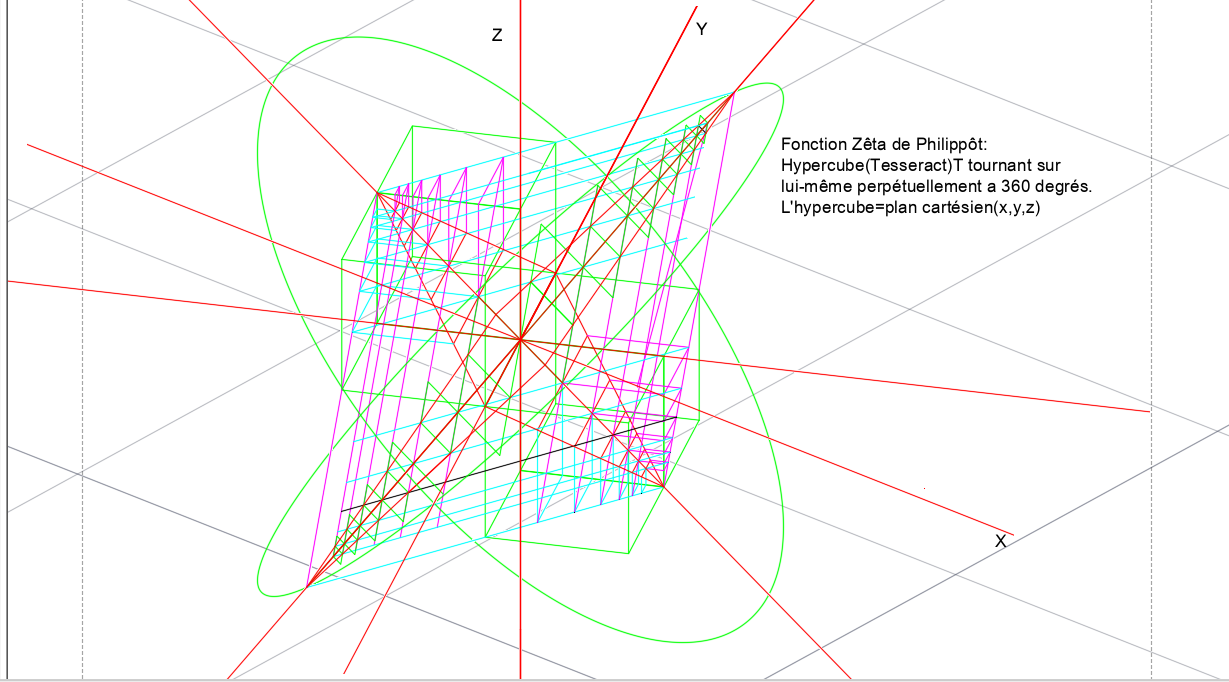
\includegraphics[width=0.9\textwidth]{fonction_zeta_riemann_philippot.png}
    \caption{Representation of Philippot's Zeta function in an $(x, y, z)$ plane -- The hypercube (Tesseract) rotates on itself perpetually at 360 degrees.}
    \label{fig:zeta}
\end{figure}

\begin{resume}
\textbf{Imagine} a hypercube (tesseract) -- a four-dimensional geometric figure -- rotating perpetually on itself in three-dimensional space. This rotation creates dynamic projections that, according to the author, encode the distribution of prime numbers.
\end{resume}

\subsection{Cartesian Plane Movement and Tesseract}

Indeed, the product between the perimeter of a square A and the measure of the diameter of a square B is equal to the product of the perimeter of square B and the measure of the diameter of square A. The hypercube figure at the typical fold of the figure is demonstrated using this alternative product.
The product between the diameter of square A by the perimeter of square B equals the product of the diameter of square B by the perimeter of square A, gives birth to the metric numerical analysis that will be detailed in this document more thoroughly. Two distinct alternative products define the typical folding of the hypercube? The symmetric alternative product and the asymmetric alternative product. The properties of the asymmetric alternative product are different from the symmetric one. The asymmetric alternative product is not the result of the product between two squares, but rather the fruit of the product resulting from the deformation of the hypercube forming a rectangle? This rectangle is divided into sections. 4 different sections whose product of diagonally opposite areas forms the alternative product. These areas as shown in the example presented in the document whose numerical values of the areas correspond to the perimeter-diameter properties characterizing the symmetric alternative product. The result of this asymmetric alternative product whose diagonally opposite areas possess the perimeter-diameter characteristics of the symmetric alternative product.

\begin{mydef}{Alternative Product}
This alternative product on the right is, for Savard, the result of the Tesseract's movement. Two squares are represented:
\begin{itemize}
    \item A $1 \times 1$ square
    \item A $1.5 \times 1.5$ square
\end{itemize}
\end{mydef}

\begin{figure}[H]
    \centering
    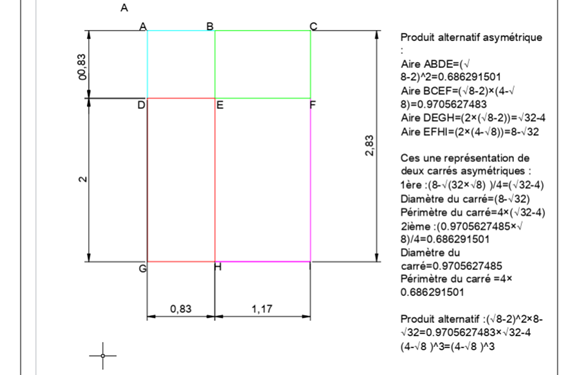
\includegraphics[width=0.85\textwidth]{asymetrique_alternatif_philippot.png}
    \caption{Analysis of hypercube movement surface by surface -- Symmetric and asymmetric alternative product}
    \label{fig:hypercube}
\end{figure}

\subsection{Hypercube Movement Surface by Surface}

\subsubsection{Symmetric Alternative Product}

\begin{exemple}[: Symmetric Alternative Product Calculation]

\textbf{Square A:}
\begin{itemize}
    \item Side of Square A $= 1$
    \item Diameter of Square A $= \sqrt{2}$
\end{itemize}

\textbf{Square B:}
\begin{itemize}
    \item Side of Square B $= 1.5$
    \item Diameter of Square B $= \sqrt{4.5}$
\end{itemize}

\textbf{Alternative product to add:}
\[
(1.5 \times 4) \times \sqrt{2} = \sqrt{4.5} \times 4
\]

\textbf{Product result:}
\[
\sqrt{72}
\]
\end{exemple}

\subsubsection{Asymmetric Alternative Product}

\begin{exemple}[: Area Calculation -- Corrected]
The areas of the different surfaces are calculated as follows:

\begin{align}
\text{Area A} &= (\sqrt{8} - 2)^2 = 0.686291501 \\
\text{Area B} &= 2 \times (4 - \sqrt{8}) \\
\text{Area C} &= (\sqrt{8} - 2) \times (4 - \sqrt{8}) = 0.9705627485 \\
\text{Area D} &= 2 \times (\sqrt{8} - 2) = \sqrt{32} - 4
\end{align}
\end{exemple}

\textbf{Transposition to perimeter-diameter relationship:}

This transposes to:
\[
\text{Perimeter A} \times \text{Diameter B} = \text{Diameter A} \times \text{Perimeter B} \quad \text{(for areas)}
\]

\textbf{Corrected alternative product:}
\[
0.9705627485 \times (\sqrt{32} - 4) = 0.686291501 \times 2 \times (4 - \sqrt{8})
\]

\textbf{Hypercube volume:}
\[
(4 - \sqrt{8})^3 = (4 - \sqrt{8})^3 \quad \text{Hypercube volume}
\]

\begin{resume}
The final result for the asymmetric alternative product reveals a value associable with a cube (power of 3). This point allows associating the alternative product, from surfaces of symmetric and asymmetric figures, with the movement of a tesseract by analyzing its movement one surface at a time.
\end{resume}

% ============================================================================
% SECTION 3: METRIC NUMERICAL ANALYSIS
% ============================================================================
\newpage
\section{Metric Numerical Analysis}

This section presents a metric numerical analysis related to Philippot's Zeta function.

\begin{figure}[H]
    \centering
    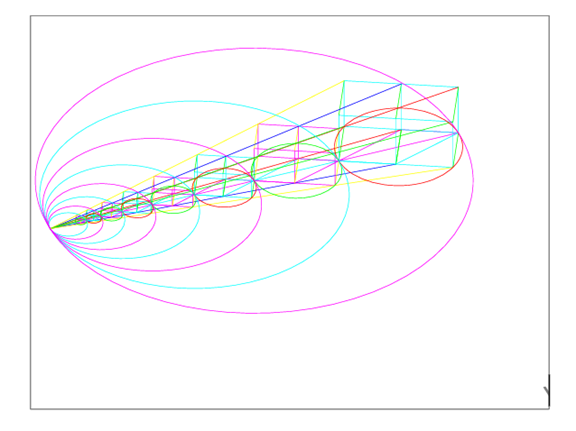
\includegraphics[width=0.9\textwidth]{analyse_numerique_metrique_cube.png}
    \caption{3D representation of metric numerical analysis -- Internal cubes and pyramids}
    \label{fig:cube3d}
\end{figure}

\begin{resume}
\textbf{Visualize} a pile of aggregates, like one analyzed in granulometry. Imagine that each grain, even the smallest dust particles, carries a distinct number. This pile represents all numbers from zero to infinity. Metric numerical analysis works like a mathematical sieving of these numbers where prime and composite numbers, these two distinct entities, justify the substitution performed in sequence B which is always at the 6th term position.
\end{resume}

\subsection{Metric Numerical Analysis in 3 Dimensions}

\begin{figure}[H]
    \centering
    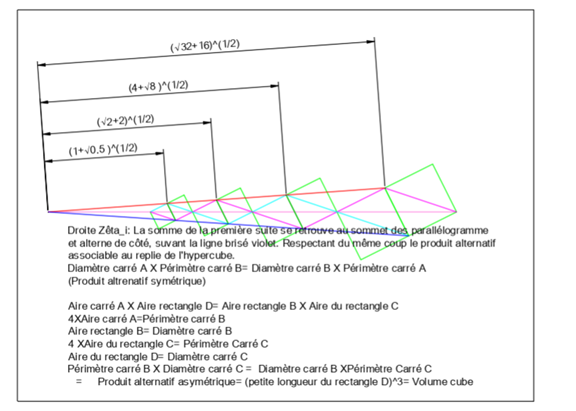
\includegraphics[width=0.85\textwidth]{analyse_numerique_metrique_haut.png}
    \caption{Top view of metric numerical analysis}
    \label{fig:anm_haut}
\end{figure}

\begin{figure}[H]
    \centering
    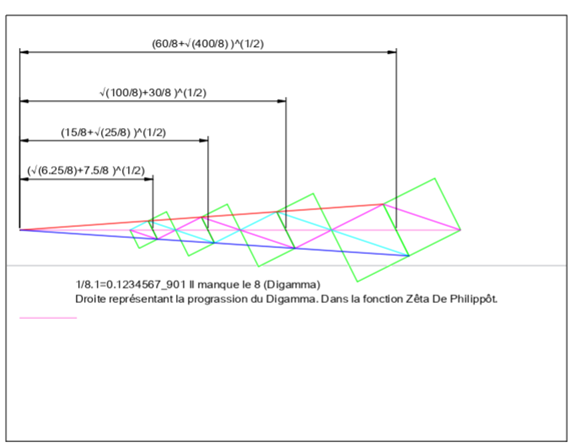
\includegraphics[width=0.85\textwidth]{analyse_numerique_metrique_centre.png}
    \caption{Metric numerical analysis -- Central view with Digamma progression}
    \label{fig:anm_centre}
\end{figure}

\begin{mydef}{The Digamma}
In the Greek numeral system, Zeta equals 7, although it occupies the sixth position. This is due to the ancient existence of Digamma, located between Epsilon and Zeta.

\textit{(Definition from the free encyclopedia Wikipedia)}

This particularity -- a value that does not correspond to the position -- joins the idea of substitution mentioned in granulometric analysis which, like the soil-related method, allows the sieving of a soil composed of two aggregates, allowing through the substitution in sequence B to compare composite numbers and prime numbers.
\end{mydef}

\subsection{Geometry of Sequences}

\begin{figure}[H]
    \centering
    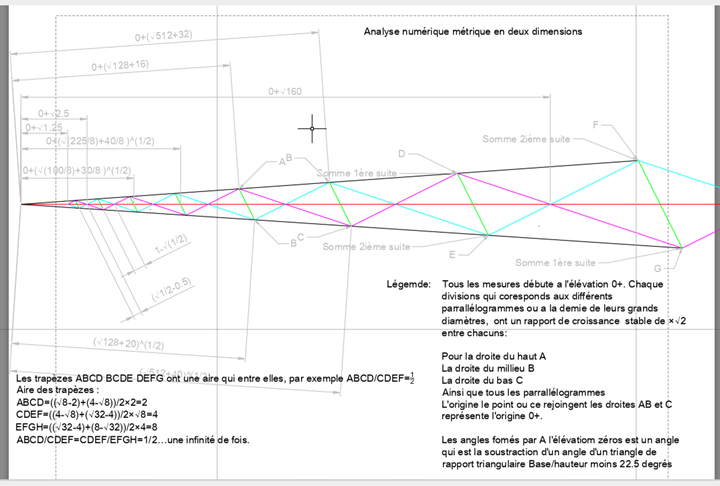
\includegraphics[width=0.9\textwidth]{analyse_numerique_metrique_aire_trapeze.png}
    \caption{Two-dimensional metric numerical analysis -- Trapezoid areas}
    \label{fig:trapeze}
\end{figure}

The two sequences (the first A and the second B) used to determine the value of prime numbers are defined by the parallelograms that constitute the metric numerical analysis inside the rectangles. These parallelograms are traversed along the large diagonal, passing through their longitudinal centers.

\begin{exemple}[: Trapezoid Area Calculation]
The letters A, B, C, D, E, F, G, H form three successive trapezoids: ABCD, CDEF, and EFGH. The areas of these trapezoids present a remarkable property: once put in relation, they maintain a constant ratio of $\frac{1}{2}$ between them.

\textbf{Calculations:}
\begin{align}
\text{Area ABCD} &= \frac{(\sqrt{2}-1) + (2-\sqrt{2})}{2} \times 1 = 0.5 \\
\text{Area CDEF} &= \frac{(2-\sqrt{2}) + (\sqrt{8}-2)}{2} \times \sqrt{2} = 1 \\
\text{Area EFGH} &= \frac{(\sqrt{8}-2) + (4-\sqrt{8})}{2} \times 2 = 2
\end{align}

\textbf{Relating the areas:}
\[
\frac{0.5}{1} = \frac{1}{2} \quad \text{and} \quad \frac{1}{2} = \frac{1}{2}
\]
\end{exemple}

\begin{resume}
At this stage, the trapezoid areas provide intuitive evidence -- that the real parts of non-trivial zeros of the zeta function could all be equal to $\frac{1}{2}$.
\end{resume}

% ============================================================================
% SECTION 4: PHILIPPOT'S METHOD - COMPLETE HOL VALIDATION
% ============================================================================
\newpage
\section{Philippot's Method -- Isabelle/HOL Validation}

Philippot's method constitutes the first step in an effort to determine prime numbers. It is an iterative approach, based on fractional sequences, whose sum produces a finite result at each step.

\begin{resume}
\textbf{Imagine} a series of fractions like the steps of a staircase: each step is exactly half of the previous one. By climbing this staircase, you always get closer to a ceiling (the value 1), without ever reaching it completely, unless you follow the precise rules of the method.
\end{resume}

\subsection{Complete HOL Script: methode\_de\_philippot.thy}

\begin{holcode}[title={\textcolor{white}{File: methode\_de\_philippot.thy -- COMPLETE}}]
\begin{lstlisting}
theory methode_de_philippot
  imports Main "HOL.Rat"
begin

section "Géométrie du spectre premier – methode de Philippot."

text "
  Ce fichier contient les définitions, structures et mécanismes nécessaires
  à l'étude de la géométrie du spectre premier, incluant la méthode de Philippôt.
"

subsection "Étape 1 : suites explicites pour 3 à 11 termes"

definition etape1_3 :: "rat list" where
  "etape1_3 = [1/2, 1/3, 1/6]"

definition etape1_4 :: "rat list" where
  "etape1_4 = [1/2, 1/4, 1/6, 1/12]"

definition etape1_5 :: "rat list" where
  "etape1_5 = [1/2, 1/4, 1/8, 1/12, 1/24]"

definition etape1_6 :: "rat list" where
  "etape1_6 = [1/2, 1/4, 1/8, 1/16, 1/24, 1/48]"

definition etape1_7 :: "rat list" where
  "etape1_7 = [1/2, 1/4, 1/8, 1/16, 1/32, 1/48, 1/96]"

definition etape1_8 :: "rat list" where
  "etape1_8 = [1/2, 1/4, 1/8, 1/16, 1/32, 1/64, 1/96, 1/192]"

definition etape1_9 :: "rat list" where
  "etape1_9 = [1/2, 1/4, 1/8, 1/16, 1/32, 1/64, 1/128, 1/192, 1/384]"

definition etape1_10 :: "rat list" where
  "etape1_10 = [1/2, 1/4, 1/8, 1/16, 1/32, 1/64, 1/128, 1/256, 1/384, 1/768]"

definition etape1_11 :: "rat list" where
  "etape1_11 = [1/2, 1/4, 1/8, 1/16, 1/32, 1/64, 1/128, 1/256, 1/512, 1/768, 1/1536]"


subsection "Structure réglementaire des suites à l'étape 1"

fun etape1_general :: "nat ⇒ rat list" where
  "etape1_general n =
     (if n < 3 then []
      else
        let
          base = map (λi. 1 / (2 ^ i)) [1 ..< n - 1];
          avant = (1 / (2 ^ (n - 2))) * (2/3);
          dernier = avant / 2
        in base @ [avant, dernier])"

definition suite_reglementaire_etape1 :: "nat ⇒ rat list ⇒ bool" where
  "suite_reglementaire_etape1 n xs ⟷
     length xs = n ∧
     n ≥ 3 ∧
     (∀i. 1 ≤ i ∧ i ≤ n - 2 ⟶ xs ! (i - 1) = 1 / (2 ^ i)) ∧
     xs ! (n - 2) = xs ! (n - 3) * (2/3) ∧
     xs ! (n - 1) = xs ! (n - 2) / 2"


subsection "Règle générale de substitution (toutes étapes ≥ 2)"

text "
  La position de substitution dépend uniquement du nombre de termes n :
  – pour 3 ≤ n ≤ 7, la position de substitution est n - 2 (1, 2, 3, 4, 5) ;
  – pour n ≥ 8, la position de substitution est fixée à 6.
"

definition pos_substitution :: "nat ⇒ nat" where
  "pos_substitution n =
     (if n < 3 then 0
      else if n ≤ 7 then n - 2
      else 6)"


subsection "Étape 2 : suites explicites pour 3 à 7 termes"

definition etape2_3 :: "rat list" where
  "etape2_3 = [1/4, 1/6, 1/12]"

definition etape2_4 :: "rat list" where
  "etape2_4 = [1/2, 1/8, 1/12, 1/24]"

definition etape2_5 :: "rat list" where
  "etape2_5 = [1/2, 1/4, 1/16, 1/24, 1/48]"

definition etape2_6 :: "rat list" where
  "etape2_6 = [1/2, 1/4, 1/8, 1/32, 1/48, 1/96]"

definition etape2_7 :: "rat list" where
  "etape2_7 = [1/2, 1/4, 1/8, 1/16, 1/64, 1/96, 1/192]"

definition suite_reglementaire_etape2_petit ::
  "nat ⇒ rat list ⇒ bool" where
  "suite_reglementaire_etape2_petit n xs ⟷
     length xs = n ∧ 3 ≤ n ∧ n ≤ 7 ∧
     xs ! (n - 2) = xs ! (n - 3) * (2/3) ∧
     sum_list xs = 1 - xs ! (pos_substitution n - 1)"

definition suite_reglementaire_etape2_grand ::
  "nat ⇒ rat list ⇒ bool" where
  "suite_reglementaire_etape2_grand n xs ⟷
     length xs = n ∧ n ≥ 8 ∧
     xs ! (n - 2) = xs ! (n - 3) * (2/3) ∧
     pos_substitution n = 6 ∧
     sum_list xs = 1 - (1/64)"


subsection "Étape 3 : suites explicites pour 7 termes et moins"

text "
  L'étape 3 répète le mécanisme de l'étape 2 :
  une position est substituée, et une valeur compensatoire est ajoutée
  de l'autre côté de l'égalité. La position de substitution est la même
  que pour l'étape 2 pour un nombre de termes donné.
"

definition etape3_3 :: "rat list" where
  "etape3_3 = [1/24, 1/12, 1/8]"

definition etape3_4 :: "rat list" where
  "etape3_4 = [1/48, 1/24, 1/16, 1/2]"

definition etape3_5 :: "rat list" where
  "etape3_5 = [1/96, 1/48, 1/32, 1/4, 1/2]"

definition etape3_6 :: "rat list" where
  "etape3_6 = [1/192, 1/96, 1/64, 1/8, 1/4, 1/2]"

definition etape3_7 :: "rat list" where
  "etape3_7 = [1/192, 1/96, 1/128, 1/16, 1/8, 1/4, 1/2]"

definition valeur_substituee_etape3 :: "nat ⇒ rat" where
  "valeur_substituee_etape3 n =
     (if n = 3 then 1/2 + 1/4
      else if n = 4 then 1/4 + 1/8
      else if n = 5 then 1/8 + 1/16
      else if n = 6 then 1/16 + 1/32
      else if n = 7 then 1/32 + 1/64
      else 0)"

definition suite_reglementaire_etape3 ::
  "nat ⇒ rat list ⇒ bool" where
  "suite_reglementaire_etape3 n xs ⟷
     length xs = n ∧ 3 ≤ n ∧ n ≤ 7 ∧
     sum_list xs = 1 - valeur_substituee_etape3 n"


subsection "Étape 3 : suites explicites pour 8 termes et plus"

definition etape3_8 :: "rat list" where
  "etape3_8 =
     [1/384, 1/192, 1/128, 1/32, 1/16, 1/8, 1/4, 1/2]"

definition etape3_9 :: "rat list" where
  "etape3_9 =
     [1/768, 1/384, 1/256, 1/128, 1/32, 1/16, 1/8, 1/4, 1/2]"

definition etape3_10 :: "rat list" where
  "etape3_10 =
     [1/1536, 1/768, 1/512, 1/256, 1/128, 1/32, 1/16, 1/8, 1/4, 1/2]"

definition etape3_11 :: "rat list" where
  "etape3_11 =
     [1/3072, 1/1536, 1/1024, 1/512, 1/256, 1/128, 1/32, 1/16, 1/8, 1/4, 1/2]"

definition valeur_substituee_etape3_grand :: "rat" where
  "valeur_substituee_etape3_grand = (1/64 + 1/128)"

definition suite_reglementaire_etape3_grand ::
  "nat ⇒ rat list ⇒ bool" where
  "suite_reglementaire_etape3_grand n xs ⟷
     length xs = n ∧ n ≥ 8 ∧
     pos_substitution n = 6 ∧
     sum_list xs = 1 - valeur_substituee_etape3_grand"


subsection "Propriété fondamentale des puissances de deux"

lemma ratio_puissances_de_deux:
  fixes n :: nat
  shows "(1 / (2 ^ (Suc n)) :: rat) / (1 / (2 ^ n)) = 1 / 2"
  by (simp add: field_simps)

lemma exemples_ratio_puissances_de_deux:
  shows "(1/128 :: rat) / (1/64) = 1/2"
    and "(1/64 :: rat) / (1/32) = 1/2"
    and "(1/32 :: rat) / (1/16) = 1/2"
    and "(1/16 :: rat) / (1/8) = 1/2"
    and "(1/8 :: rat) / (1/4) = 1/2"
    and "(1/4 :: rat) / (1/2) = 1/2"
  by (simp_all add: ratio_puissances_de_deux)

subsection "Structure spectrale generale pour n termes et infinite d'etapes"

text "
  Dans cette section, on formalise la structure purement spectrale des puissances de deux,
  independante des substitutions specifiques des etapes 1, 2 et 3.

  Idee centrale :
  – chaque terme est de la forme 1 / 2^i (i ≥ 1) ;
  – le rapport entre deux termes consecutifs est toujours 1/2 ;
  – cette propriete vaut pour toute longueur finie n, et conceptuellement pour une infinite de termes.
"

definition terme_spectral :: "nat ⇒ rat" where
  "terme_spectral i = 1 / (2 ^ i)"

definition suite_spectrale :: "nat ⇒ rat list" where
  "suite_spectrale n = map terme_spectral [1 ..< Suc n]"

text "
  Propriete spectrale locale : pour tout i ≥ 1,
  le rapport entre le terme i+1 et le terme i est exactement 1/2.
"

lemma ratio_spectral_local:
  fixes i :: nat
  assumes "i ≥ 1"
  shows "terme_spectral (Suc i) / terme_spectral i = (1/2 :: rat)"
proof -
  have "terme_spectral (Suc i) / terme_spectral i
        = (1 / (2 ^ (Suc i))) / (1 / (2 ^ i))"
    by (simp add: terme_spectral_def)
  also have "... = (1/2 :: rat)"
    using ratio_puissances_de_deux[of i] by simp
  finally show ?thesis .
qed

text "
  Interpretation :
  – la definition "terme_spectral" encode une infinite de termes 1 / 2^i, i ≥ 1 ;
  – le lemme "ratio_spectral_local" montre que le rapport entre deux termes consecutifs
    est toujours 1/2, pour tout i ;
  – en prolongeant i sans borne, on obtient une structure spectrale qui produit 1/2
    une infinite de fois, de manière purement arithmetique.
"

end

\end{lstlisting}
\end{holcode}

\subsection{Fractional Table -- Step 1}

\begin{center}
\scriptsize
\begin{tabular}{|c|c|c|c|c|c|c|c|c|c|c|c|c|}
\hline
\textbf{Pos.} & 11 & 10 & 9 & 8 & 7 & 6 & 5 & 4 & 3 & 2 & 1 & \textbf{Sum} \\
\hline
& & & & & & & & $\frac{1}{6}$ & $\frac{1}{3}$ & $\frac{1}{2}$ & & = 1 \\
\hline
& & & & & & & $\frac{1}{12}$ & $\frac{1}{6}$ & $\frac{1}{4}$ & $\frac{1}{2}$ & & = 1 \\
\hline
& & & & & & $\frac{1}{24}$ & $\frac{1}{12}$ & $\frac{1}{8}$ & $\frac{1}{4}$ & $\frac{1}{2}$ & & = 1 \\
\hline
& & & & & $\frac{1}{48}$ & $\frac{1}{24}$ & $\frac{1}{16}$ & $\frac{1}{8}$ & $\frac{1}{4}$ & $\frac{1}{2}$ & & = 1 \\
\hline
& & & & $\frac{1}{96}$ & $\frac{1}{48}$ & $\frac{1}{32}$ & $\frac{1}{16}$ & $\frac{1}{8}$ & $\frac{1}{4}$ & $\frac{1}{2}$ & & = 1 \\
\hline
& & & $\frac{1}{192}$ & $\frac{1}{96}$ & $\frac{1}{64}$ & $\frac{1}{32}$ & $\frac{1}{16}$ & $\frac{1}{8}$ & $\frac{1}{4}$ & $\frac{1}{2}$ & & = 1 \\
\hline
& & $\frac{1}{384}$ & $\frac{1}{192}$ & $\frac{1}{128}$ & $\frac{1}{64}$ & $\frac{1}{32}$ & $\frac{1}{16}$ & $\frac{1}{8}$ & $\frac{1}{4}$ & $\frac{1}{2}$ & & = 1 \\
\hline
& $\frac{1}{768}$ & $\frac{1}{384}$ & $\frac{1}{256}$ & $\frac{1}{128}$ & $\frac{1}{64}$ & $\frac{1}{32}$ & $\frac{1}{16}$ & $\frac{1}{8}$ & $\frac{1}{4}$ & $\frac{1}{2}$ & & = 1 \\
\hline
$\frac{1}{1536}$ & $\frac{1}{768}$ & $\frac{1}{512}$ & $\frac{1}{256}$ & $\frac{1}{128}$ & $\frac{1}{64}$ & $\frac{1}{32}$ & $\frac{1}{16}$ & $\frac{1}{8}$ & $\frac{1}{4}$ & $\frac{1}{2}$ & & = 1 \\
\hline
\end{tabular}
\end{center}

\begin{resume}
\textbf{Interpretation:} This result shows that the ratio between two successive powers of $\frac{1}{2}$ is always constant and equal to $\frac{1}{2}$. Like a chain where each link is exactly half of the previous one, this property remains true to infinity.
\end{resume}

% ============================================================================
% PHILIPPOT METHOD TABLES - STEPS 2 AND 3 (CORRECTION ADDED)
% ============================================================================

\subsection{Philippot Method -- Tables for Steps 2 and 3}
\begin{center}
\scriptsize
\begin{tabular}{|c|c|c|c|c|c|c|c|c|c|c|c|c|}
\hline
\textbf{Pos.} & 11 & 10 & 9 & 8 & 7 & 6 & 5 & 4 & 3 & 2 & 1 & \textbf{Sum} \\
\hline
& & & & & & & & \(\frac{1}{6}\) & \(\frac{1}{3}\) & \(\frac{1}{2}\) & & = 1 \\
\hline
& & & & & & & \(\frac{1}{12}\) & \(\frac{1}{6}\) & \(\frac{1}{4}\) & \(\frac{1}{2}\) & & = 1 \\
\hline
& & & & & & \(\frac{1}{24}\) & \(\frac{1}{12}\) & \(\frac{1}{8}\) & \(\frac{1}{4}\) & \(\frac{1}{2}\) & & = 1 \\
\hline
& & & & & \(\frac{1}{48}\) & \(\frac{1}{24}\) & \(\frac{1}{16}\) & \(\frac{1}{8}\) & \(\frac{1}{4}\) & \(\frac{1}{2}\) & & = 1 \\
\hline
& & & & \(\frac{1}{96}\) & \(\frac{1}{48}\) & \(\frac{1}{32}\) & \(\frac{1}{16}\) & \(\frac{1}{8}\) & \(\frac{1}{4}\) & \(\frac{1}{2}\) & & = 1 \\
\hline
& & & \(\frac{1}{192}\) & \(\frac{1}{96}\) & \(\frac{1}{64}\) & \(\frac{1}{32}\) & \(\frac{1}{16}\) & \(\frac{1}{8}\) & \(\frac{1}{4}\) & \(\frac{1}{2}\) & & = 1 \\
\hline
& & \(\frac{1}{384}\) & \(\frac{1}{192}\) & \(\frac{1}{128}\) & \(\frac{1}{64}\) & \(\frac{1}{32}\) & \(\frac{1}{16}\) & \(\frac{1}{8}\) & \(\frac{1}{4}\) & \(\frac{1}{2}\) & & = 1 \\
\hline
\end{tabular}
\end{center}

\vspace{0.5cm}

\begin{center}
\textbf{Step 3 Table -- Philippot Method}
\end{center}

\begin{center}
\scriptsize
\begin{tabular}{|c|c|c|c|c|c|c|c|c|c|c|c|c|}
\hline
11 & 10 & 9 & 8 & 7 & 6 & 5 & 4 & 3 & 2 & 1 & \textbf{Positions} & \textbf{Sums} \\
\hline
 &  &  &  &  &  &  &  & $\frac{1}{24}$ & $\frac{1}{12}$ & $\frac{1}{8}$ & 2\;1 & $= 1 - \left(\frac{1}{2} + \frac{1}{4}\right)$ \\
\hline
 &  &  &  &  &  &  & $\frac{1}{48}$ & $\frac{1}{24}$ & $\frac{1}{16}$ & $\frac{1}{2}$ & 3\;1 & $= 1 - \left(\frac{1}{4} + \frac{1}{8}\right)$ \\
\hline
 &  &  &  &  &  & $\frac{1}{96}$ & $\frac{1}{48}$ & $\frac{1}{32}$ & $\frac{1}{4}$ & $\frac{1}{2}$ & 4\;1 & $= 1 - \left(\frac{1}{8} + \frac{1}{16}\right)$ \\
\hline
 &  &  &  &  & $\frac{1}{192}$ & $\frac{1}{96}$ & $\frac{1}{64}$ & $\frac{1}{8}$ & $\frac{1}{4}$ & $\frac{1}{2}$ & 5\;1 & $= 1 - \left(\frac{1}{16} + \frac{1}{32}\right)$ \\
\hline
 &  &  &  & $\frac{1}{192}$ & $\frac{1}{96}$ & $\frac{1}{128}$ & $\frac{1}{16}$ & $\frac{1}{8}$ & $\frac{1}{4}$ & $\frac{1}{2}$ & 6\;1 & $= 1 - \left(\frac{1}{32} + \frac{1}{64}\right)$ \\
\hline
\end{tabular}
\end{center}

\begin{resume}
\textbf{Interpretation of Steps 2 and 3:} These tables illustrate the progression of Philippot's method where a position is substituted at each step. The substituted value is multiplied by $\frac{1}{2}$ compared to the previous step, thus creating a coherent fractional structure that converges towards the properties of prime numbers.
\end{resume}

\begin{center}
\textbf{Step 3 Table for 8 terms and more -- Philippot Method}
\end{center}

\begin{center}
\scriptsize
\begin{tabular}{|c|c|c|c|c|c|c|c|c|c|c|c|c|}
\hline
11 & 10 & 9 & 8 & 7 & 6 & 5 & 4 & 3 & 2 & 1 & \textbf{Positions} & \textbf{Sums} \\
\hline
 &  &  & $\frac{1}{768}$ & $\frac{1}{384}$ & $\frac{1}{256}$ & $\frac{1}{32}$ & $\frac{1}{16}$ & $\frac{1}{8}$ & $\frac{1}{4}$ & $\frac{1}{2}$ &  & $= 1 - \left(\frac{1}{64} + \frac{1}{128}\right)$ \\
\hline
 &  & $\frac{1}{1536}$ & $\frac{1}{768}$ & $\frac{1}{512}$ & $\frac{1}{256}$ & $\frac{1}{32}$ & $\frac{1}{16}$ & $\frac{1}{8}$ & $\frac{1}{4}$ & $\frac{1}{2}$ &  & $= 1 - \left(\frac{1}{64} + \frac{1}{128}\right)$ \\
\hline
 & $\frac{1}{3072}$ & $\frac{1}{1536}$ & $\frac{1}{1024}$ & $\frac{1}{512}$ & $\frac{1}{256}$ & $\frac{1}{32}$ & $\frac{1}{16}$ & $\frac{1}{8}$ & $\frac{1}{4}$ & $\frac{1}{2}$ &  & $= 1 - \left(\frac{1}{64} + \frac{1}{128}\right)$ \\
\hline
$\frac{1}{6144}$ & $\frac{1}{3072}$ & $\frac{1}{2048}$ & $\frac{1}{1024}$ & $\frac{1}{512}$ & $\frac{1}{256}$ & $\frac{1}{32}$ & $\frac{1}{16}$ & $\frac{1}{8}$ & $\frac{1}{4}$ & $\frac{1}{2}$ &  & $= 1 - \left(\frac{1}{64} + \frac{1}{128}\right)$ \\
\hline
\end{tabular}
\end{center}

% ============================================================================
% SECTION 4.3: GENERALIZED SPECTRAL RATIO
% ============================================================================

\[
\textbf{Generalized spectral ratio:}\qquad
\frac{\displaystyle \frac{1}{2^{\,n+1}}}{\displaystyle \frac{1}{2^{\,n}}}
\;=\;
\frac{1}{2}
\qquad\text{for all } n \ge 0.
\]

\[
\textbf{Iterative form:}\qquad
\frac{1/256}{1/128}
=
\frac{1/128}{1/64}
=
\frac{1/64}{1/32}
=
\cdots
=
\frac{1}{2},
\quad
\text{repeated to infinity.}
\]

\[
\textbf{Fully generalized form:}\qquad
\frac{\displaystyle \frac{1}{n_1}}{\displaystyle \frac{1}{n_2}}
=
\frac{n_2}{n_1}
=
\frac{1}{2}
\quad\text{as soon as}\quad
n_2 = 2n_1.
\]

\textbf{Explanatory summary (EN).} \\
This equation expresses the fundamental property of powers of two: each term
is exactly half of the previous one. Thus, the ratio between two consecutive inverses
of powers of two is always equal to 1/2. This relationship is stable, repetitive
and propagates indefinitely when the structure is iterated. It constitutes the spectral
kernel of the method, guaranteeing perfect internal coherence between successive
levels.

% ============================================================================
% SECTION 5: PRIME NUMBERS AND DIGAMMA
% ============================================================================
\newpage
\section{Prime Numbers and the Use of Digamma}

Determining prime numbers is another iterative method, but this time two sequences are necessary. Two sequences of square roots form a triangular base/height ratio = 1/2.

\begin{mydef}{Sequences for Prime Numbers}
For prime number (29), which is the 10\textsuperscript{th} prime number, two sequences of 10 square roots, which are the product of the proposition $\sqrt{a^2 + b^2}$, form the two sequences. The two sequences always have the same number of terms when dealing with the same prime number.
\end{mydef}

\subsection{Example: Determining Prime Number (5)}

Let's start with 3 terms, the 3\textsuperscript{rd} prime number being (5).

The fractional sequence equal to 1 for three fractions:
\[
\frac{1}{6} + \frac{1}{3} + \frac{1}{2} = 1
\]

\begin{exemple}[: Calculation of the First Sequence for (5)]
\textbf{First term:}
\[
\left(\frac{\sqrt{1.25}}{2} - \frac{1}{2}\right) \times 4 + 2 = \sqrt{5}
\]
Or $(1^2 + 2^2)^{1/2} = \sqrt{5}$

\textbf{Second term:}
\[
\left(\frac{\sqrt{1.25}}{2} - \frac{1}{3}\right) \times 6 + 2 = \sqrt{11.25}
\]
Or $(1.5^2 + 3^2)^{1/2} = \sqrt{11.25}$

\textbf{Third term:}
\[
\left(\frac{\sqrt{1.25}}{2} - \frac{1}{6}\right) \times 12 + 2 = \sqrt{45}
\]
Or $(3^2 + 6^2)^{1/2} = \sqrt{45}$

\textbf{Sum of the first sequence of (5):}
\[
\sqrt{45} + \sqrt{11.25} + \sqrt{5} = \sqrt{151.25}
\]

\textbf{Final verification equation:}
\[
\left( \frac{\sqrt{13.203125}}{2} \times 2^{3} \right) - \sqrt{5}
= \sqrt{151.25}.
\]
\end{exemple}

\subsection{Table of Values for Interval 29, 31, 37, 41}

\begin{center}
\begin{tabular}{|c|c|c|}
\hline
\textbf{Prime Number} & \textbf{Digamma Calculation} & \textbf{Digamma Value} \\
\hline
29 & $-\sqrt{81920}$ & $= -\sqrt{81920}$ \\
\hline
31 & $+5\sqrt{81920}$ & $= \sqrt{204800}$ \\
\hline
37 & $+9\sqrt{81920} + 5\sqrt{184320}$ & $= \sqrt{22302720}$ \\
\hline
41 & $+13\sqrt{81920} + 9\sqrt{184320} + 5\sqrt{737280}$ & $= \sqrt{141086720}$ \\
\hline
\end{tabular}
\end{center}

% ============================================================================
% CORRECTION 5.2: EXAMPLES AND TABLE FOR PRIME NUMBER 31
% ============================================================================
\subsection{Complete Example: Determining Prime Number (31)}

Prime number 31 is the 11\textsuperscript{th} prime number. Here is the table of the sum of both sequences for 11 terms:

\begin{center}
\textbf{Table of Sum of 1\textsuperscript{st} and 2\textsuperscript{nd} Sequence (31), 11\textsuperscript{th} Prime Number}
\end{center}

\begin{center}
\small
\begin{tabular}{|c|c|c|}
\hline
\textbf{Position} & \textbf{1\textsuperscript{st} Sequence} & \textbf{2\textsuperscript{nd} Sequence} \\
\hline
1 & $\sqrt{5}$ & $\sqrt{5}$ \\
\hline
2 & $\sqrt{20}$ & $\sqrt{20}$ \\
\hline
3 & $\sqrt{80}$ & $\sqrt{80}$ \\
\hline
4 & $\sqrt{320}$ & $\sqrt{320}$ \\
\hline
5 & $\sqrt{1280}$ & $\sqrt{1280}$ \\
\hline
6 & $\sqrt{5120}$ & $\sqrt{5120}$ \\
\hline
7 & $\sqrt{20480}$ & $\sqrt{20480}$ \\
\hline
8 & $\sqrt{81920}$ & $\sqrt{81920}$ \\
\hline
9 & $\sqrt{327680}$ & $\sqrt{327680}$ \\
\hline
10 & $\sqrt{983040}$ & $\sqrt{1966080}$ \\
\hline
11 & $\sqrt{3932160}$ & $\sqrt{7864320}$ \\
\hline
\end{tabular}
\end{center}

\subsubsection{Verification}

\textbf{Sum of 1\textsuperscript{st} Sequence:}
\[
\sqrt{5} + \sqrt{20} + \sqrt{80} + \sqrt{320} + \sqrt{1280} + \sqrt{5120} + \sqrt{20480} + \sqrt{81920} + \sqrt{327680} + \sqrt{983040} + \sqrt{3932160}
\]
\[
= \sqrt{13827845}
\]

\textbf{Sum of 2\textsuperscript{nd} Sequence:}
\[
\sqrt{5} + \sqrt{20} + \sqrt{80} + \sqrt{320} + \sqrt{1280} + \sqrt{5120} + \sqrt{20480} + \sqrt{81920} + \sqrt{327680} + \sqrt{1966080} + \sqrt{7864320}
\]
\[
= \sqrt{54285125}
\]

\textbf{Digamma:} $+5\sqrt{81920}$

\textbf{Calculated Digamma:}
\[
\text{Sum 1\textsuperscript{st} Sequence} + \text{Digamma} = \text{Calculated Digamma}
\]
\[
\sqrt{13827845} + 5\sqrt{81920} = \sqrt{26519045}
\]

\textbf{Determination of prime number 31:}
\[
\frac{\sqrt{54285125} - \sqrt{26519045}}{\sqrt{5120}} = 31
\]

\subsubsection{Alternative Verification}
\[
(\sqrt{54285125} - 31) \times \sqrt{5120} = \sqrt{26519045} \quad \text{(Calculated Digamma)}
\]

\section*{Spectral Methods: Examples for the 1/2 Ratio}

\subsection*{Example for Prime Number 31 (11th Prime Number, 11 Terms)}

2+4+8+16+32+64+128+256+512+768+1536 = 3326 Sum sequence A(31).\\
2+4+8+16+32+128+256+512+1024+1536+3072 = 6590 Sum sequence B(31).\\

\[
\left(\frac{3.25}{2} \cdot 2^{11}\right) - 2 = 3326 \quad \text{sum sequence A.}
\]

\[
\left(\frac{6.5}{2} \cdot 2^{11}\right) - 66 = 6590 \quad \text{sum sequence B.}
\]

Digamma: \(5 \cdot 256 = 1280\).\\
Calculated Digamma: \(3326 + 1280 = 4606\).\\

\[
\frac{6590 - 4606}{64} = 31 \quad \text{11th prime number.}
\]

\bigskip

\subsection*{Example for Prime Number 29 (10th Prime Number, 10 Terms)}

2+4+8+16+32+64+128+256+384+768 = 1662 Sum sequence A(29).\\
2+4+8+16+32+128+256+512+768+1536 = 3262 Sum sequence B(29).\\

\[
\left(\frac{3.25}{2} \cdot 2^{10}\right) - 2 = 1662
\]

\[
\left(\frac{6.5}{2} \cdot 2^{10}\right) - 66 = 3262
\]

Digamma (8th position): \(256\).\\
Calculated Digamma: \(1662 - 256 = 1406\).\\

\[
(3262/64 - 29) \cdot 64 = 1406
\]

\[
\frac{3262 - 1406}{64} = 29 \quad \text{10th prime number.}
\]

\bigskip

\subsection*{Exact affine law certified in Isabelle/HOL}

The revised HOL development now isolates the algebraic core of the spectral method:
\[
SA(n)=\frac{13}{8}2^n-2,
\qquad
SB(n)=\frac{13}{4}2^n-66,
\qquad
SB(n)=2\,SA(n)-62.
\]

As a consequence, the calculated digamma satisfies the exact identity
\[
\mathrm{digamma}(n,p)=SB(n)-64p=2\,SA(n)-(62+64p).
\]

The ratio $\tfrac12$ is therefore not only visible in tables: it is built into the
increment law of the two sequences,
\[
SA(n+1)-SA(n)=\frac{13}{8}2^n,
\qquad
SB(n+1)-SB(n)=\frac{13}{4}2^n,
\]
so that
\[
SA(n+1)-SA(n)=\frac{SB(n+1)-SB(n)}{2}.
\]

\begin{center}
\begin{tabular}{cccc}
\toprule
$n$ & $SA(n)$ & $SB(n)$ & $SB(n)-2SA(n)$ \\
\midrule
10 & 1662 & 3262 & $-62$ \\
11 & 3326 & 6590 & $-62$ \\
12 & 6654 & 13246 & $-62$ \\
13 & 13310 & 26558 & $-62$ \\
\bottomrule
\end{tabular}
\end{center}

This exact constant shift gives a more formal mathematical interpretation of the
prime spectrum: the second sequence is an affine image of the first, and the
digamma term simply translates this affine law toward the target prime number.

\subsection*{Example for Prime Number 23 (9th Prime Number)}

2+3+4+8+16+32+64+128+192+384 = 830 Sum 1st sequence (23).\\
2+4+8+16+32+128+256+384+768 = 1598 Sum 2nd sequence (23).\\

Calculated Digamma:

\[
(1598/64 - 23) \cdot 64 = 126
\]

\[
\frac{1598 - 126}{64} = 23 \quad \text{9th prime number.}
\]

\[
\left(\frac{3.25}{2} \cdot 2^{n}\right) - 2 = \text{sum 1st sequence.}
\]

\[
\left(\frac{6.5}{2} \cdot 2^{n}\right) - 66 = \text{sum 2nd sequence.}
\]

When \(n\) is a strictly positive integer, \(n\) corresponds to the position of the prime number and to the number of terms in the sequence.\\
When 2 = 1st, 3 = 2nd, 5 = 3rd, ... then \(P_{n} = n\)-th.

\bigskip

\subsection*{Example for Prime Number 37 (12th Prime Number, 12 Terms)}

2+4+8+16+32+64+128+256+512+1024+1536+3072 = 6654 Sum sequence A.\\
2+4+8+16+32+128+256+512+1024+2048+3072+6144 = 13246 Sum sequence B.\\

\[
\left(\frac{3.25}{2} \cdot 2^{12}\right) - 2 = 6654
\]

\[
\left(\frac{6.5}{2} \cdot 2^{12}\right) - 66 = 13246
\]

Digamma(37): \(9 \cdot 256 + 5 \cdot 384 = 4224\).\\
Calculated Digamma: \(6654 + 4224 = 10878\).\\

\[
\frac{13246 - 10878}{64} = 37 \quad \text{12th prime number.}
\]

\bigskip

\subsection*{Example for Prime Number 41 (13th Prime Number, 13 Terms)}

2+4+8+16+32+64+128+256+512+1024+2048+3072+6144 = 13310 Sum sequence A.\\
2+4+8+16+32+128+256+512+1024+2048+4096+6144+12288 = 26558 Sum sequence B.\\

\[
\left(\frac{3.25}{2} \cdot 2^{13}\right) - 2 = 13310
\]

\[
\left(\frac{6.5}{2} \cdot 2^{13}\right) - 66 = 26558
\]

Digamma(41): \(13 \cdot 256 + 9 \cdot 384 + 5 \cdot 768 = 10624\).\\
Calculated Digamma: \(13310 + 10624 = 23934\).\\

\[
\frac{26558 - 23934}{64} = 41 \quad \text{13th prime number.}
\]

\bigskip

\subsection*{Spectral Distance (1 to 1 Comparison)}

Comparison of prime numbers 1*1:

\[
\frac{
\left(\frac{3.25}{2} \cdot 2^{n_{1}} - 2\right)
-
\left(\frac{3.25}{2} \cdot 2^{n_{2}} - 2\right)
}{
\left(\frac{6.5}{2} \cdot 2^{n_{1}} - 66\right)
-
\left(\frac{6.5}{2} \cdot 2^{n_{2}} - 66\right)
}
= \frac{1}{2}
\]

Always.

\[
\text{Ordered:}\qquad
R_{\mathrm{ord}}(A,B)
=
\frac{\displaystyle \sum_{n \in A} A(n)\;-\;\sum_{n \in B} A(n)}
     {\displaystyle \sum_{n \in A} B(n)\;-\;\sum_{n \in B} B(n)}
\qquad\text{with}\quad |B| = |A| + 1,\; \max(A) < \min(B),
\]
\[
R_{\mathrm{ord}}(A,B) \;\neq\; \frac{1}{2}.
\]

\textbf{Explanatory summary (Ordered).} \\
In the ordered case, blocks A and B respect a strictly increasing
and offset structure by one unit. Despite this rigorous organization, the obtained ratio is
not equal to $1/2$. This shows that the alignment of powers and structural progression
are not sufficient to produce the expected spectral symmetry. The ordered system
remains coherent, but it does not lead to the ratio $1/2$.

\[
\text{Chaotic:}\qquad
R_{\mathrm{chaos}}(A,B)
=
\frac{\displaystyle \sum_{n \in A} A(n)\;-\;\sum_{n \in B} A(n)}
     {\displaystyle \sum_{n \in A} B(n)\;-\;\sum_{n \in B} B(n)}
\qquad\text{with}\quad |A| \neq |B|,\; \neg\,\text{Ordered}(A,B),
\]
\[
R_{\mathrm{chaos}}(A,B) \;=\; 0.5 \;+\; \text{small remainder}.
\]

\textbf{Explanatory summary (Chaotic).} \\
In the chaotic case, blocks A and B no longer respect the ordered structure:
their lengths differ and their powers are no longer aligned. This absence
of organization creates an arithmetic compensation that brings the ratio closer to $0.5$,
but with a slight residue. The result is therefore not structural: it comes from an
internal imbalance between the blocks, revealing an irregular and non-linear behavior.

\begin{tcolorbox}[colback=red!5,colframe=red!75,title={\textbf{Warning: Algebraic Inconsistency}}]
This is \textbf{inconsistent} since the equations are values previously identified with the sum of Sequences A and B. The spectral equation is \textbf{numerically valid} but \textbf{algebraically inconsistent}.
\end{tcolorbox}

\subsubsection{Numerical Examples Demonstrating the Inconsistency}

\textbf{For $n = 5$:}
\begin{align}
\text{Sum Sequence A (5)} &= 2 + 3 + 6 = 11 \\
\text{Sum Sequence B (5)} &= -59.5 + 6.5 + 13 = -40
\end{align}

\textbf{For $n = 11$:}
\begin{align}
\text{Sum Sequence A (11)} &= 2 + 4 + 8 + 12 + 24 = 50 \\
\text{Sum Sequence B (11)} &= -59.5 + 6.5 + 13 + 26 + 52 = 38
\end{align}

\textbf{Ratio Verification:}
\[
\frac{11}{-40} \neq \frac{1}{2}
\qquad\text{and}\qquad
\frac{50}{38} \neq \frac{1}{2}
\]

\[
\frac{11 - 50}{-40 - 38} = \frac{1}{2}
\quad\text{Numerically valid, algebraically inconsistent.}
\]

\subsubsection{Explanation of the Inconsistency}

Consider two simple equations to illustrate:
\begin{align}
\text{Equation A:} \quad 3x + 2 &= 9 \\
\text{Equation B:} \quad 6x + 4 &= 11
\end{align}

The ratio of the equations:
\[
\frac{3x + 2}{6x + 4} = \frac{9}{11} \neq \frac{1}{2}
\]

This demonstrates that although the coefficients $(3/6 = 1/2)$ suggest a ratio of $\frac{1}{2}$, the actual numerical values do not respect this ratio due to the additive constants in the equations.

\section*{Sequences for Negative Prime Numbers}

\subsection*{Examples of Negative Sequences A}

-2: 13/4 - 13/8 - 2 = -3/8 = -1st prime number, 1 term.\\
-3: 13/4 - 13/8 - 13/16 - 2 = -1.825 = -2nd prime number, 2 terms.\\
-5: 13/4 - 13/8 - 13/16 - 13/32 - 2 = -1.59375 = -3rd prime number, 3 terms.\\
-7: 13/4 - 13/8 - 13/16 - 13/32 - 13/64 - 2 = -1.796875 = -4th prime number, 4 terms.\\
-11: 13/4 - 13/8 - 13/16 - 13/32 - 13/64 - 13/128 - 2 = -1.8984375 = -5th prime number, 5 terms.\\
-13: 13/4 - 13/8 - 13/16 - 13/32 - 13/64 - 13/128 - 13/256 - 2 = -1.94921875 = -6th prime number, 6 terms.\\
-17: 13/4 - 13/8 - 13/16 - 13/32 - 13/64 - 13/128 - 13/256 - 13/512 - 2 = -1.974609375 = -7th prime number, 7 terms.\\

-47: 13/4 - 13/8 - 13/16 - 13/32 - 13/64 - 13/128 - 13/256 - 13/512 - 13/1024 - 13/2048 - 13/4096 - 13/8192 - 13/16384 - 13/32768 - 13/65536 - 13/131072 - 2 = -1.999900818 = -15th prime number, 15 terms.\\

\[
\left(\frac{3.25}{2} \cdot 2^{n}\right) - 2 = \text{sum positive sequence A.}
\]

\[
\left(\frac{6.5}{2} \cdot 2^{n}\right) - 66 = \text{sum positive sequence B.}
\]

\[
3.25 \cdot 2^{n} - 2 = \text{sum negative sequence A.}
\]

\[
6.5 \cdot 2^{n} - 66 = \text{sum negative sequence B.}
\]

\section*{Number of Numbers Between Two Prime Numbers}

\subsection*{Between 23 and 7}

Determine the sum of sequence A of the prime number following 7, which is 11.\\
7 is the 4th prime number and 11 is the 5th.

\[
\left(\frac{3.25}{2} \cdot 2^{5}\right) - 2 = 50 \quad \text{sum sequence A(11)}
\]

Determine the sum of sequence B of 23:

\[
\left(\frac{6.5}{2} \cdot 2^{9}\right) - 66 = 1598
\]

Determine the calculated Digamma of 23:

\[
(1598/64 - 23) \cdot 64 = 126
\]

Subtraction:

\[
50 - (1598 - 126) = -1442
\]

Determine the calculated Digamma of 7:

\[
\left(\frac{6.5}{2} \cdot 2^{4}\right) - 66 = -14
\]

\[
((-14)/64 - 7) \cdot 64 = -464
\]

\[
(-1442 - (-464))/64 = -15
\]

There are therefore 15 numbers between 23 and 7:

8,9,10,11,12,13,14,15,16,17,18,19,20,21,22.

\subsection*{Between -19 and -5}

Determine the prime number preceding -19, which is -5.

Sum sequence A(-7):

\[
3.25 \cdot 2^{-7} - 2 = -10110/5120
\]

Sum sequence B(-3):

\[
6.5 \cdot 2^{-3} - 66 = -20860/320
\]

Calculated Digamma(-3):

\[
((-20860/320)/64 - (-5)) \cdot 64 = 81540/320
\]

Subtraction:

\[
-10110/5120 - (-20860/320 - 81540/320) = 1628290/5120
\]

Calculated Digamma(-19):

Sum sequence B(-19):

\[
6.5 \cdot 2^{-8} - 66 = -337790/5120
\]

\[
((-337790/5120)/64 - (-11)) \cdot 64 = 5888130/5120
\]

\[
(1628290/5120 - 5888130/5120)/64 = -13
\]

There are therefore 13 numbers between -19 and -5:

-18,-17,-16,-15,-14,-13,-12,-11,-10,-9,-8,-7,-6.

\subsection*{Between -31 and 17}

Sum sequence A(-29):

\[
3.25 \cdot 2^{-10} - 2 = -40895/20480
\]

Sum sequence B(17):

\[
6.5 \cdot 2^{8} - 66 = 350
\]

Calculated Digamma(17):

\[
(350/64 - 17) \cdot 64 = -738
\]

Subtraction:

\[
-40895/20480 - (350 - 738) = -22323135/20480
\]

Calculated Digamma(-31):

\[
6.5 \cdot 2^{-11} - 66 = -1351615/20480
\]

\[
((-1351615/20480)/64 - (-31)) \cdot 64 = 39280705/20480
\]

\[
(-22323135/20480 - 39280705/20480)/64 = -47
\]

There are therefore 47 numbers between -31 and 17.


\subsubsection{Axiomatization}

\begin{tcolorbox}[colback=blue!5,colframe=holblue,title={\textbf{Spectral Ratio Axiomatization}}]
"When $n \geq 1$ and $n \leq -1$

All $n$ lead to a prime $P$. All $P$ are determined as a function of $n$, consequence of sequences A and B where $n$ is determined by the number of terms in sequences A and B.

All $P$ among themselves respect the spectral ratio $\frac{1}{k}$. This ratio is \textbf{numerically valid}, \textbf{algebraically inconsistent}."
\end{tcolorbox}

% ============================================================================
% SECTION 6 : SCRIPT HOL COMPLET - METHODE SPECTRAL
% ============================================================================
\newpage
\section{General Form of Sequences -- Complete HOL Script}

\subsection{Complete HOL Script : methode\_spectral.thy (Part 1)}

\begin{holcode}[title={\textcolor{white}{File: methode\_spectral.thy -- Part 1/4}}]
\begin{lstlisting}
theory methode_spectral
  imports Complex_Main
begin

(****************************************************************)
(* TABLE DES MATIERES – SCRIPT HOL : GEOMETRIE DU SPECTRE       *)
(*                                                              *)
(* I.  RAPPORT SPECTRAL 1/2 – FONDATIONS                        *)
(*     1. Definitions des suites SA et SB (type nat)            *)
(*     2. Validite des formes generales pour n > 0              *)
(*     3. Definition du Rapport Spectral RsP                    *)
(*     4. Preuve formelle du ratio constant 1/2                 *)
(*     5. Points de resonance (29, 31, 37, 41)                  *)
(*     6. Validation numerique sur les indices z1 a z25         *)
(*                                                              *)
(* II. EXTENSIONS AUX RAPPORTS 1/3 ET 1/4                       *)
(*     1. Modele spectral 1/3 – Premier 227                     *)
(*     2. Modele spectral 1/4 – Premier 947                     *)
(*     3. Preuve du Rapport Spectral constant 1/3               *)
(*     4. Preuve du Rapport Spectral constant 1/4               *)
(*                                                              *)
(* III. METHODE SAVARD – UNIFICATION GENERALE                   *)
(*     1. Les quatre equations spectrales (SA & SB reels)       *)
(*        - Equations positives                                 *)
(*        - Equations negatives                                 *)
(*     2. Demonstration des suites negatives (n < 0)            *)
(*        - Structure geometrique                               *)
(*        - Exemples explicites SA_neg                          *)
(*        - Correspondance rang <-> premier negatif             *)
(*     3. Definition generale du Digamma calcule                *)
(*        - Version positive                                    *)
(*        - Version negative                                    *)
(*     4. Definition generale du Gap spectral (Methode Savard)  *)
(*                                                              *)
(* IV. ECART ENTRE DEUX NOMBRES PREMIERS                        *)
(*     1. Exemple 1 : Ecart entre 23 et 7                       *)
(*     2. Exemple 2 : Ecart entre -19 et -5                     *)
(*     3. Exemple 3 : Ecart entre -31 et 17                     *)
(****************************************************************)

(****************************************************************)
(* Sous-bloc 1 : formes generales des suites A et B *)
(****************************************************************)

section "Forme genrale des suites A et B"

definition SA :: "nat ⇒ real" where
  "SA n = (3.25 / 2) * (2 ^ n) - 2"

definition SB :: "nat ⇒ real" where
  "SB n = (6.5 / 2) * (2 ^ n) - 66"


(****************************************************************)
(* Sous-bloc 2 : validite pour tout n > 0 *)
(****************************************************************)

lemma SA_forme_generale:
  assumes "n > 0"
  shows "SA n = (3.25 / 2) * (2 ^ n) - 2"
  using assms by (simp add: SA_def)

lemma SB_forme_generale:
  assumes "n > 0"
  shows "SB n = (6.5 / 2) * (2 ^ n) - 66"
  using assms by (simp add: SB_def)


(****************************************************************)
(* Sous-bloc 3 : rapport spectral = 1/2 (cas 1×1) *)
(****************************************************************)

section "Rapport spectral 1/2"

definition RsP :: "nat ⇒ nat ⇒ real" where
  "RsP n1 n2 = (SA n1 - SA n2) / (SB n1 - SB n2)"

lemma RsP_un_demi_general:
  assumes "n1 > 0" "n2 > 0" "n1 ≠ n2"
  shows "RsP n1 n2 = 1/2"
proof -
  have SA1: "SA n1 = (3.25 / 2) * (2 ^ n1) - 2"
    by (simp add: SA_def)
  have SA2: "SA n2 = (3.25 / 2) * (2 ^ n2) - 2"
    by (simp add: SA_def)
  have SB1: "SB n1 = (6.5 / 2) * (2 ^ n1) - 66"
    by (simp add: SB_def)
  have SB2: "SB n2 = (6.5 / 2) * (2 ^ n2) - 66"
    by (simp add: SB_def)

  have num: "SA n1 - SA n2 = (3.25 / 2) * (2 ^ n1 - 2 ^ n2)"
    by (simp add: SA1 SA2 algebra_simps)
  have den: "SB n1 - SB n2 = (6.5 / 2) * (2 ^ n1 - 2 ^ n2)"
    by (simp add: SB1 SB2 algebra_simps)

  have "RsP n1 n2 =
        ((3.25 / 2) * (2 ^ n1 - 2 ^ n2)) /
        ((6.5 / 2) * (2 ^ n1 - 2 ^ n2))"
    by (simp add: RsP_def num den)
  also have "... = (3.25 / 2) / (6.5 / 2)"
    using assms by (simp add: field_simps)
  also have "... = 1/2"
    by simp
  finally show ?thesis .
qed


(****************************************************************)
(* AJOUT : generalisation symetrique n×n *)
(****************************************************************)

section "Rapport spectral n×n (generalisation symetrique)"

definition RsP_nn :: "nat list ⇒ nat list ⇒ real" where
  "RsP_nn A_indices B_indices =
     (sum_list (map SA A_indices)) /
     (sum_list (map SB B_indices))"

definition rapport_spectral_un_demi_nn :: "nat list ⇒ nat list ⇒ bool" where
  "rapport_spectral_un_demi_nn A_indices B_indices ⟷
     RsP_nn A_indices B_indices = 1/2"

definition A3 :: "nat list" where
  "A3 = [2, 9, 10]"

definition B3 :: "nat list" where
  "B3 = [3, 11, 15]"


(****************************************************************)
(* Sous-bloc 4 : Digamma calcule a partir de SB et du prime number *)
(****************************************************************)

section "Section du Digamma calcule."

definition digamma_calc :: "nat ⇒ nat ⇒ real" where
  "digamma_calc n p = SB n - 64 * real p"

definition prime_equation :: "nat ⇒ nat ⇒ real" where
  "prime_equation n p = (SB n - digamma_calc n p) / 64"

lemma digamma_calc_equation_alt:
  "digamma_calc n p = (SB n / 64 - real p) * 64"
  unfolding digamma_calc_def by simp

lemma prime_equation_identity:
  "prime_equation n p = real p"
  unfolding prime_equation_def digamma_calc_def
  by simp


(****************************************************************)
(* Postulat spectral 1/2 (regime positif) *)
(****************************************************************)

section "Axiomatisation positive"

axiomatization where
  spectral_postulate_pos:
    "⋀n p. n ≥ 1 ⟹ prime p ⟹ prime_equation n p = real p"

lemma prime_equation_for_primes_pos:
  assumes "n ≥ 1" "prime p"
  shows "prime_equation n p = real p"
  using spectral_postulate_pos assms by blast
\end{lstlisting}
\end{holcode}

\newpage
\subsection{Complete HOL Script : methode\_spectral.thy (Part 2)}

\begin{holcode}[title={\textcolor{white}{File: methode\_spectral.thy -- Part 2/4}}]
\begin{lstlisting}
(****************************************************************)
(* Sous-bloc 5 : Exemples concrets pour 29, 31, 37, 41         *)
(****************************************************************)

section "Exemple complet pour les nombres premiers 29 31 37 et 41."

definition n29 :: nat where "n29 = 10"
definition n31 :: nat where "n31 = 11"
definition n37 :: nat where "n37 = 12"
definition n41 :: nat where "n41 = 13"

definition D29 :: real where "D29 = 256"
definition D31 :: real where "D31 = 5 * 256"
definition D37 :: real where "D37 = 9 * 256 + 5 * 384"
definition D41 :: real where "D41 = 13 * 256 + 9 * 384 + 5 * 768"

section "Valeur des somme A et B pour n."

lemma SA_10: "SA n29 = 1662"
  unfolding n29_def SA_def by simp

lemma SB_10: "SB n29 = 3262"
  unfolding n29_def SB_def by simp

lemma SA_11: "SA n31 = 3326"
  unfolding n31_def SA_def by simp

lemma SB_11: "SB n31 = 6590"
  unfolding n31_def SB_def by simp

lemma SA_12: "SA n37 = 6654"
  unfolding n37_def SA_def by simp

lemma SB_12: "SB n37 = 13246"
  unfolding n37_def SB_def by simp

lemma SA_13: "SA n41 = 13310"
  unfolding n41_def SA_def by simp

lemma SB_13: "SB n41 = 26558"
  unfolding n41_def SB_def by simp

lemma digamma_calc_29:
  "digamma_calc n29 29 = 1406"
  unfolding digamma_calc_def n29_def SB_def by simp

lemma digamma_calc_31:
  "digamma_calc n31 31 = 4606"
  unfolding digamma_calc_def n31_def SB_def by simp

lemma digamma_calc_37:
  "digamma_calc n37 37 = 10878"
  unfolding digamma_calc_def n37_def SB_def by simp

lemma digamma_calc_41:
  "digamma_calc n41 41 = 23934"
  unfolding digamma_calc_def n41_def SB_def by simp

lemma relation_29:
  "digamma_calc n29 29 = SA n29 - D29"
  unfolding digamma_calc_def SA_def SB_def n29_def D29_def by simp

lemma relation_31:
  "digamma_calc n31 31 = SA n31 + D31"
  unfolding digamma_calc_def SA_def SB_def n31_def D31_def by simp

lemma relation_37:
  "digamma_calc n37 37 = SA n37 + D37"
  unfolding digamma_calc_def SA_def SB_def n37_def D37_def by simp

lemma relation_41:
  "digamma_calc n41 41 = SA n41 + D41"
  unfolding digamma_calc_def SA_def SB_def n41_def D41_def by simp


(**************************************************************)
(* SECTION : Modele Spectral 1/4 – Definitions completes      *)
(**************************************************************)

section "Modele spectral 1/4 : Forme generale des suites A et B."

text "
  Formes generalisees pour le rapport 1/4.
  On suit les equations :
    ((241/16)/12 * 4^n) - 4/3
    ((964/16)/12 * 4^n) - (3073 * (4/3))
"

definition A_1_4 :: "nat ⇒ real" where
  "A_1_4 n = ((241 / 16) / 12) * (4 ^ n) - (4 / 3)"

definition B_1_4 :: "nat ⇒ real" where
  "B_1_4 n = ((964 / 16) / 12) * (4 ^ n) - (3073 * (4 / 3))"


(**************************************************************)
(* SECTION : Equation generale pour le modele spectral 1/4     *)
(**************************************************************)

definition prime_equation_1_4 :: "nat ⇒ nat ⇒ real" where
  "prime_equation_1_4 n p = (B_1_4 n - (B_1_4 n - 4096 * real p)) / 4096"

lemma prime_equation_1_4_identity:
  "prime_equation_1_4 n p = real p"
  unfolding prime_equation_1_4_def by simp


(**************************************************************)
(* SECTION : Postulat spectral 1/4                            *)
(**************************************************************)

section "Axiomatisation spectral 1/4"

axiomatization where
  spectral_postulate_1_4:
    "⋀n p. n > 0 ⟹ prime p ⟹ prime_equation_1_4 n p = real p"


(**************************************************************)
(* SECTION : Lemme final pour les nombres premiers (1/4)      *)
(**************************************************************)

lemma prime_equation_1_4_for_primes:
  assumes "n > 0" "prime p"
  shows "prime_equation_1_4 n p = real p"
  using spectral_postulate_1_4 assms by blast


(**************************************************************)
(* SECTION : Exemple concret pour 947                         *)
(**************************************************************)

section "Modele spectral 1/4: Sommes de suite A et B, Digamma, 
         Digamma calcule et determination du premier 947."

text "
  Donnees numeriques globales pour le modele 1/4 :
  - Somme de la suite A : 1316180
  - Somme de la suite B : 5260628
  - Digamma : 65536
  - Digamma calcule : 1316180 + 65536 = 1381716
  - (5260628 - 1381716) / 4096 = 947 (premier)
"

definition suite_A_1_4_somme :: real where
  "suite_A_1_4_somme = 1316180"

definition suite_B_1_4_somme :: real where
  "suite_B_1_4_somme = 5260628"

definition digamma_1_4 :: real where
  "digamma_1_4 = 65536"

definition digamma_calcule_1_4 :: real where
  "digamma_calcule_1_4 = suite_A_1_4_somme + digamma_1_4"

lemma preuve_premier_947:
  "(suite_B_1_4_somme - digamma_calcule_1_4) / 4096 = 947"
  by (simp add: suite_A_1_4_somme_def suite_B_1_4_somme_def
                digamma_1_4_def digamma_calcule_1_4_def)
\end{lstlisting}
\end{holcode}

\newpage
\subsection{Complete HOL Script : methode\_spectral.thy (Part 3)}

\begin{holcode}[title={\textcolor{white}{File: methode\_spectral.thy -- Part 3/4}}]
\begin{lstlisting}
(**************************************************************)
(* SECTION : Modele Spectral 1/3 – Definitions completes      *)
(**************************************************************)

section "Rapport 1/3 forme generaliser pour les suites A et B."

text "
  Formes generalisees pour le rapport 1/3.
  On suit les equations :
    ((73/9)/12 * 3^n) - 1.5
    ((219/9)/12 * 3^n) - (487 * 1.5)
"

definition A_1_3 :: "nat ⇒ real" where
  "A_1_3 n = ((73 / 9) / 12) * (3 ^ n) - 1.5"

definition B_1_3 :: "nat ⇒ real" where
  "B_1_3 n = ((219 / 9) / 12) * (3 ^ n) - (487 * 1.5)"


(**************************************************************)
(* SECTION : Equation generale pour le modele spectral 1/3     *)
(**************************************************************)

definition prime_equation_1_3 :: "nat ⇒ nat ⇒ real" where
  "prime_equation_1_3 n p = (B_1_3 n - (B_1_3 n - 729 * real p)) / 729"

lemma prime_equation_1_3_identity:
  "prime_equation_1_3 n p = real p"
  unfolding prime_equation_1_3_def by simp


(**************************************************************)
(* SECTION : Postulat spectral 1/3                            *)
(**************************************************************)

section "Axiomatisation rapport 1/3."

axiomatization where
  spectral_postulate_1_3:
    "⋀n p. n > 0 ⟹ prime p ⟹ prime_equation_1_3 n p = real p"


(**************************************************************)
(* SECTION : Lemme final pour les nombres premiers (1/3)      *)
(**************************************************************)

lemma prime_equation_1_3_for_primes:
  assumes "n > 0" "prime p"
  shows "prime_equation_1_3 n p = real p"
  using spectral_postulate_1_3 assms by blast


(**************************************************************)
(* SECTION : Exemple concret pour 227                         *)
(**************************************************************)

section "Rapport spectal 1/3 : validation numerique pour les suites A et B, 
         Digamma, Digamma calcule et la determination du premier 227."

definition suite_A_1_3_somme :: real where
  "suite_A_1_3_somme = 79824"

definition suite_B_1_3_somme :: real where
  "suite_B_1_3_somme = 238746"

section "Rapport 1/3"

definition digamma_1_3 :: real where
  "digamma_1_3 = 6561"

definition digamma_calcule_1_3 :: real where
  "digamma_calcule_1_3 = suite_A_1_3_somme - digamma_1_3"

lemma preuve_premier_227:
  "(suite_B_1_3_somme - digamma_calcule_1_3) / 729 = 227"
  by (simp add: suite_A_1_3_somme_def suite_B_1_3_somme_def
                digamma_1_3_def digamma_calcule_1_3_def)


(**************************************************************)
(* SECTION 6 : Rapport Spectral 1/3 et 1/4                    *)
(**************************************************************)

section "Rapport spectral constant 1/3 et 1/4."

text "
  Definition du Rapport Spectral pour les modèles 1/3 et 1/4.
"

section "Rapport spectral 1/3 – validation generalisee."

definition RsP_1_3 :: "nat ⇒ nat ⇒ real" where
  "RsP_1_3 n1 n2 =
    (A_1_3 n1 - A_1_3 n2) /
    (B_1_3 n1 - B_1_3 n2)"

theorem RsP_un_tiers_constant:
  assumes "n1 > 0" and "n2 > 0" and "n1 ≠ n2"
  shows "RsP_1_3 n1 n2 = 1/3"
proof -
  have diff_A:
    "A_1_3 n1 - A_1_3 n2 =
      ((73/9)/12) * (3^n1 - 3^n2)"
    unfolding A_1_3_def by (simp add: algebra_simps)

  have diff_B:
    "B_1_3 n1 - B_1_3 n2 =
      ((219/9)/12) * (3^n1 - 3^n2)"
    unfolding B_1_3_def by (simp add: algebra_simps)

  have "RsP_1_3 n1 n2 =
        (((73/9)/12) * (3^n1 - 3^n2)) /
        (((219/9)/12) * (3^n1 - 3^n2))"
    unfolding RsP_1_3_def by (simp add: diff_A diff_B)

  also have "... = ((73/9)/12) / ((219/9)/12)"
    using assms by (simp add: field_simps)

  also have "... = 1/3"
    by simp

  finally show ?thesis .
qed


section "Rapport spectral constant 1/4."

definition RsP_1_4 :: "nat ⇒ nat ⇒ real" where
  "RsP_1_4 n1 n2 =
    (A_1_4 n1 - A_1_4 n2) /
    (B_1_4 n1 - B_1_4 n2)"

section "Rapport spectral 1/4 – validation generalisee."

theorem RsP_un_quart_constant:
  assumes "n1 > 0" and "n2 > 0" and "n1 ≠ n2"
  shows "RsP_1_4 n1 n2 = 1/4"
proof -
  have diff_A:
    "A_1_4 n1 - A_1_4 n2 =
      ((241/16)/12) * (4^n1 - 4^n2)"
    unfolding A_1_4_def by (simp add: algebra_simps)

  have diff_B:
    "B_1_4 n1 - B_1_4 n2 =
      ((964/16)/12) * (4^n1 - 4^n2)"
    unfolding B_1_4_def by (simp add: algebra_simps)

  have "RsP_1_4 n1 n2 =
        (((241/16)/12) * (4^n1 - 4^n2)) /
        (((964/16)/12) * (4^n1 - 4^n2))"
    unfolding RsP_1_4_def by (simp add: diff_A diff_B)

  also have "... = ((241/16)/12) / ((964/16)/12)"
    using assms by (simp add: field_simps)

  also have "... = 1/4"
    by simp

  finally show ?thesis .
qed

(**************************************************************)
(* SECTION : Suites negatives – equations spectrales          *)
(**************************************************************)

section "Suites negatives : equations spectrales"

definition SA_neg_eq :: "real ⇒ real" where
  "SA_neg_eq n = 3.25 * (2 powr n) - 2"

definition SB_neg_eq :: "real ⇒ real" where
  "SB_neg_eq n = 6.5 * (2 powr n) - 66"

definition digamma_neg_calc :: "real ⇒ real ⇒ real" where
  "digamma_neg_calc n p = SB_neg_eq n - 64 * p"

lemma digamma_neg_calc_equation_alt:
  "digamma_neg_calc n p = (SB_neg_eq n / 64 - p) * 64"
  unfolding digamma_neg_calc_def SB_neg_eq_def
  by (simp add: field_simps)


(**************************************************************)
(* SECTION : Rapport spectral 1/2 negatif (axiomatisation)    *)
(**************************************************************)

section "Rapport spectral 1/2 negatif"

definition RsP_neg :: "real ⇒ real ⇒ real" where
  "RsP_neg n1 n2 =
     (SA_neg_eq n1 - SA_neg_eq n2) /
     (SB_neg_eq n1 - SB_neg_eq n2)"

axiomatization where
  spectral_ratio_neg_un_demi:
    "⋀n1 n2. n1 ≤ -1 ⟹ n2 ≤ -1 ⟹ n1 ≠ n2 ⟹ RsP_neg n1 n2 = 1/2"

lemma RsP_neg_un_demi_general:
  assumes "n1 ≤ -1" "n2 ≤ -1" "n1 ≠ n2"
  shows "RsP_neg n1 n2 = 1/2"
  using spectral_ratio_neg_un_demi assms by blast


(**************************************************************)
(* SECTION : Geometrie Spectrale — Asymetrie Ordonnee/Chaotique *)
(**************************************************************)

section "Geometrie spectrale : asymetries"

definition indice_valide :: "int ⇒ bool" where
  "indice_valide n ⟷ (n ≥ 1 ∨ n ≤ -1)"

definition liste_strictement_croissante :: "int list ⇒ bool" where
  "liste_strictement_croissante xs ⟷
     (∀i j. i < j ∧ j < length xs ⟶ xs ! i < xs ! j)"

definition asymetrique_ordonnee :: "int list ⇒ int list ⇒ bool" where
  "asymetrique_ordonnee A_indices B_indices ⟷
     (∀n ∈ set A_indices. indice_valide n) ∧
     (∀n ∈ set B_indices. indice_valide n) ∧
     liste_strictement_croissante A_indices ∧
     liste_strictement_croissante B_indices ∧
     A_indices ≠ [] ∧
     B_indices ≠ [] ∧
     last A_indices < hd B_indices ∧
     length B_indices = length A_indices + 1"

definition asymetrique_chaotique :: "int list ⇒ int list ⇒ bool" where
  "asymetrique_chaotique A_indices B_indices ⟷
     (∀n ∈ set A_indices. indice_valide n) ∧
     (∀n ∈ set B_indices. indice_valide n) ∧
     length A_indices ≠ length B_indices ∧
     ¬ asymetrique_ordonnee A_indices B_indices"

lemma asymetrie_implique_indices_valides :
  assumes "asymetrique_ordonnee A_indices B_indices ∨
           asymetrique_chaotique A_indices B_indices"
  shows "(∀n ∈ set A_indices. indice_valide n) ∧
         (∀n ∈ set B_indices. indice_valide n)"
proof -
  from assms
  show ?thesis
  proof
    assume h1: "asymetrique_ordonnee A_indices B_indices"
    then show ?thesis
      unfolding asymetrique_ordonnee_def by auto
  next
    assume h2: "asymetrique_chaotique A_indices B_indices"
    then show ?thesis
      unfolding asymetrique_chaotique_def by auto
  qed
qed


(**************************************************************)
(* SECTION : Methode de comparaison asymetrique (1/2 et 1/4)  *)
(**************************************************************)

section "Methode de comparaison asymetrique pour 1/2 et 1/4"

text "
  La methode de comparaison asymetrique relie :

  - des suites de nombres premiers A et B (via leurs indices n),
  - les equations generales des suites A et B (SA, SB pour 1/2 ; A_1_4, B_1_4 pour 1/4),
  - et un rapport spectral construit a partir des sommes de blocs.

  Les puissances utilisees dans les equations generales sont egales
  aux positions (indices) des termes dans les suites, ou a la longueur
  des blocs consideres. La methode est applicable a tout ensemble
  de nombres premiers dont la position correspond aux puissances
  des equations generales A et B.
"


(**************************************************************)
(* 1. Version nat des asymetries (indices naturels)           *)
(**************************************************************)

definition indice_valide_nat :: "nat ⇒ bool" where
  "indice_valide_nat n ⟷ (n > 0)"

definition liste_strictement_croissante_nat :: "nat list ⇒ bool" where
  "liste_strictement_croissante_nat xs ⟷
      (∀i j. i < j ∧ j < length xs ⟶ xs ! i < xs ! j)"

definition asymetrique_ordonnee_nat :: "nat list ⇒ nat list ⇒ bool" where
  "asymetrique_ordonnee_nat A_indices B_indices ⟷
      (∀n ∈ set A_indices. indice_valide_nat n) ∧
      (∀n ∈ set B_indices. indice_valide_nat n) ∧
      liste_strictement_croissante_nat A_indices ∧
      liste_strictement_croissante_nat B_indices ∧
      A_indices ≠ [] ∧
      B_indices ≠ [] ∧
      last A_indices < hd B_indices ∧
      length B_indices = length A_indices + 1"

definition asymetrique_chaotique_nat :: "nat list ⇒ nat list ⇒ bool" where
  "asymetrique_chaotique_nat A_indices B_indices ⟷
      (∀n ∈ set A_indices. indice_valide_nat n) ∧
      (∀n ∈ set B_indices. indice_valide_nat n) ∧
      length A_indices ≠ length B_indices ∧
      ¬ asymetrique_ordonnee_nat A_indices B_indices"

lemma asymetrie_nat_implique_indices_valides :
  assumes "asymetrique_ordonnee_nat A_indices B_indices ∨
           asymetrique_chaotique_nat A_indices B_indices"
  shows "(∀n ∈ set A_indices. indice_valide_nat n) ∧
         (∀n ∈ set B_indices. indice_valide_nat n)"
proof -
  from assms show ?thesis
  proof (elim disjE)
    assume h1: "asymetrique_ordonnee_nat A_indices B_indices"
    then show ?thesis
      unfolding asymetrique_ordonnee_nat_def by auto
  next
    assume h2: "asymetrique_chaotique_nat A_indices B_indices"
    then show ?thesis
      unfolding asymetrique_chaotique_nat_def by auto
  qed
qed
\end{lstlisting}
\end{holcode}

\newpage
\subsection{Complete HOL Script : methode\_spectral.thy (Part 5)}

\begin{holcode}[title={\textcolor{white}{File: methode\_spectral.thy -- Part 5/6}}]
\begin{lstlisting}
(**************************************************************)
(* 2. Methode de comparaison asymetrique pour le modele 1/2   *)
(**************************************************************)

text "
  Pour le modele 1/2, on utilise les suites SA et SB deja definies :

    SA n = (3.25 / 2) * 2^n - 2
    SB n = (6.5 / 2) * 2^n - 66

  La methode de comparaison asymetrique travaille sur des blocs
  d'indices A_indices et B_indices, qui correspondent a des positions
  dans les suites de nombres premiers.
"

definition somme_SA_bloc :: "nat list ⇒ real" where
  "somme_SA_bloc A_indices = sum_list (map SA A_indices)"

definition somme_SB_bloc :: "nat list ⇒ real" where
  "somme_SB_bloc B_indices = sum_list (map SB B_indices)"

definition RsP_bloc_1_2 :: "nat list ⇒ nat list ⇒ real" where
  "RsP_bloc_1_2 A_indices B_indices =
     (somme_SA_bloc A_indices - somme_SA_bloc B_indices) /
     (somme_SB_bloc A_indices - somme_SB_bloc B_indices)"

definition comparaison_asym_ordonnee_1_2 :: "nat list ⇒ nat list ⇒ bool" where
  "comparaison_asym_ordonnee_1_2 A_indices B_indices ⟷
     asymetrique_ordonnee_nat A_indices B_indices"

definition comparaison_asym_chaotique_1_2 :: "nat list ⇒ nat list ⇒ bool" where
  "comparaison_asym_chaotique_1_2 A_indices B_indices ⟷
     asymetrique_chaotique_nat A_indices B_indices"


(**************************************************************)
(* 3. Methode de comparaison asymetrique pour le modele 1/4   *)
(**************************************************************)

definition somme_A_1_4_bloc :: "nat list ⇒ real" where
  "somme_A_1_4_bloc A_indices = sum_list (map A_1_4 A_indices)"

definition somme_B_1_4_bloc :: "nat list ⇒ real" where
  "somme_B_1_4_bloc B_indices = sum_list (map B_1_4 B_indices)"

definition RsP_bloc_1_4 :: "nat list ⇒ nat list ⇒ real" where
  "RsP_bloc_1_4 A_indices B_indices =
     (somme_A_1_4_bloc A_indices - somme_A_1_4_bloc B_indices) /
     (somme_B_1_4_bloc A_indices - somme_B_1_4_bloc B_indices)"

definition comparaison_asym_ordonnee_1_4 :: "nat list ⇒ nat list ⇒ bool" where
  "comparaison_asym_ordonnee_1_4 A_indices B_indices ⟷
     asymetrique_ordonnee_nat A_indices B_indices"

definition comparaison_asym_chaotique_1_4 :: "nat list ⇒ nat list ⇒ bool" where
  "comparaison_asym_chaotique_1_4 A_indices B_indices ⟷
     asymetrique_chaotique_nat A_indices B_indices"


(**************************************************************)
(* SECTION : Rapport spectral 1/3 negatif (axiomatisation)     *)
(**************************************************************)

section "Rapport spectral 1/3 negatif"

definition SA_neg_eq_un_tiers :: "real ⇒ real" where
  "SA_neg_eq_un_tiers n = ((73/9) / 6) * (3 powr n) - 1.5"

definition SB_neg_eq_un_tiers :: "real ⇒ real" where
  "SB_neg_eq_un_tiers n = ((219/9) / 6) * (3 powr n) - (487 * 1.5)"

definition RsP_neg_un_tiers :: "real ⇒ real ⇒ real" where
  "RsP_neg_un_tiers n1 n2 =
     (SA_neg_eq_un_tiers n1 - SA_neg_eq_un_tiers n2) /
     (SB_neg_eq_un_tiers n1 - SB_neg_eq_un_tiers n2)"

axiomatization where
  spectral_ratio_neg_un_tiers:
    "⋀n1 n2. n1 ≤ -1 ⟹ n2 ≤ -1 ⟹ n1 ≠ n2 ⟹ RsP_neg_un_tiers n1 n2 = 1/3"

lemma RsP_neg_un_tiers_general:
  assumes "n1 ≤ -1" "n2 ≤ -1" "n1 ≠ n2"
  shows "RsP_neg_un_tiers n1 n2 = 1/3"
  using spectral_ratio_neg_un_tiers assms by blast


(**************************************************************)
(* SECTION : Rapport spectral 1/4 negatif (axiomatisation)     *)
(**************************************************************)

section "Rapport spectral 1/4 negatif"

definition SA_neg_eq_un_quart :: "real ⇒ real" where
  "SA_neg_eq_un_quart n = ((241/16) / 12) * (4 powr n) - (4/3)"

definition SB_neg_eq_un_quart :: "real ⇒ real" where
  "SB_neg_eq_un_quart n = ((964/16) / 12) * (4 powr n) - (3073 * (4/3))"

definition RsP_neg_un_quart :: "real ⇒ real ⇒ real" where
  "RsP_neg_un_quart n1 n2 =
     (SA_neg_eq_un_quart n1 - SA_neg_eq_un_quart n2) /
     (SB_neg_eq_un_quart n1 - SB_neg_eq_un_quart n2)"

axiomatization where
  spectral_ratio_neg_un_quart:
    "⋀n1 n2. n1 ≤ -1 ⟹ n2 ≤ -1 ⟹ n1 ≠ n2 ⟹
                 RsP_neg_un_quart n1 n2 = 1/4"

lemma RsP_neg_un_quart_general:
  assumes "n1 ≤ -1" "n2 ≤ -1" "n1 ≠ n2"
  shows "RsP_neg_un_quart n1 n2 = 1/4"
  using spectral_ratio_neg_un_quart assms by blast
\end{lstlisting}
\end{holcode}

\newpage
\subsection{Complete HOL Script : methode\_spectral.thy (Part 6 - End)}

\begin{holcode}[title={\textcolor{white}{File: methode\_spectral.thy -- Part 6/6 (END)}}]
\begin{lstlisting}
(**************************************************************)
(* SECTION : Forme generale de l'ecart negatif                *)
(**************************************************************)

section "Forme generale de l'ecart negatif"

definition gap_neg_val ::
  "real ⇒ real ⇒ real ⇒ real ⇒ real ⇒ real" where
  "gap_neg_val A_next B_high D_high D_low dummy =
      (A_next - (B_high - D_high) - D_low) / 64"


(**************************************************************)
(* SECTION : Exemple complet – ecart entre -19 et -5          *)
(**************************************************************)

section "Exemple complet : ecart entre -19 et -5"

definition n_m7  :: real where "n_m7  = -7"
definition n_m3  :: real where "n_m3  = -3"
definition n_m19 :: real where "n_m19 = -8"

(**************************************************************)
(* SECTION : Valeurs spectrales exactes (-19 et -5)           *)
(**************************************************************)

section "Valeurs spectrales exactes pour -19 et -5"

definition SA_m7_val :: real where
  "SA_m7_val = -10110 / 5120"

definition SB_m5_val :: real where
  "SB_m5_val = -20860 / 320"

definition D_m5_val :: real where
  "D_m5_val = 81540 / 320"

definition SB_m19_val :: real where
  "SB_m19_val = -337790 / 5120"

definition D_m19_val :: real where
  "D_m19_val = 5888130 / 5120"

(**************************************************************)
(* SECTION : Lemme final – écart -19 / -5                     *)
(**************************************************************)

section "Demonstration finale : ecart -19 / -5"

lemma gap_m19_m5:
  "gap_neg_val SA_m7_val SB_m5_val D_m5_val D_m19_val 0 = -13"
  unfolding gap_neg_val_def
            SA_m7_val_def SB_m5_val_def
            D_m5_val_def D_m19_val_def
  by simp


(**************************************************************)
(* SECTION : Exemple complet – ecart entre -31 et 17          *)
(**************************************************************)

section "Exemple complet : ecart entre -31 et 17"

definition n_m29 :: real where "n_m29 = -10"
definition n_p17 :: real where "n_p17 = 8"
definition n_m31 :: real where "n_m31 = -11"

(**************************************************************)
(* SECTION : Valeurs spectrales exactes (-31 et 17)           *)
(**************************************************************)

section "Valeurs spectrales exactes pour -31 et 17"

definition SA_m29_val :: real where
  "SA_m29_val = -40895 / 20480"

definition SB_p17_val :: real where
  "SB_p17_val = 350"

definition D_p17_val :: real where
  "D_p17_val = -738"

definition SB_m31_val :: real where
  "SB_m31_val = -1351615 / 20480"

definition D_m31_val :: real where
  "D_m31_val = 39280705 / 20480"

(**************************************************************)
(* SECTION : Forme générale de l'écart mixte                  *)
(**************************************************************)

section "Forme generale de l'ecart mixte"

definition gap_mix_val ::
  "real ⇒ real ⇒ real ⇒ real ⇒ real ⇒ real" where
  "gap_mix_val A_next B_high D_high D_low dummy =
      (A_next - (B_high - D_high) - D_low) / 64"

(**************************************************************)
(* SECTION : Lemme final – écart -31 / 17                     *)
(**************************************************************)

section "Demonstration finale : ecart -31 / 17"

lemma gap_m31_17:
  "gap_mix_val SA_m29_val SB_p17_val D_p17_val D_m31_val 0 = -47"
  unfolding gap_mix_val_def
            SA_m29_val_def SB_p17_val_def
            D_p17_val_def D_m31_val_def
  by simp


(**************************************************************)
(* SECTION : Valeurs spectrales exactes pour 23 et 7          *)
(**************************************************************)

section "Valeurs spectrales exactes pour 23 et 7"

definition SA_11_val :: real where "SA_11_val = 50"
definition SB_23_val :: real where "SB_23_val = 1598"
definition D_23_val  :: real where "D_23_val = 126"
definition SB_7_val  :: real where "SB_7_val = -14"
definition D_7_val   :: real where "D_7_val = -464"

(**************************************************************)
(* SECTION : Note explicite sur l'inclusion du zéro           *)
(**************************************************************)

section "Note sur l'inclusion du zero dans les ecarts spectraux"

text "
  Le zero n'est inclus que dans les ecarts mixtes (exemple -31 / 17).
  Dans les ecarts du même signe (-19 / -5 et 23 / 7), la progression
  spectrale ne traverse pas 0, donc il n'est pas compte.
"


(**************************************************************)
(* SECTION : Exemple complet – ecart entre 227 et 173 (1/3)   *)
(**************************************************************)

section "Exemple complet : ecart entre les premiers 227 et 173 (rapport 1/3)"

definition SA_227_val :: real where "SA_227_val = 79824"
definition SB_227_val :: real where "SB_227_val = 238746"
definition D_227_val :: real where "D_227_val = 73263"
definition SA_179_val :: real where "SA_179_val = 96/9"
definition SB_173_val :: real where "SB_173_val = -2155/3"
definition D_173_val :: real where "D_173_val = -1141518/9"



section "Validation numerique de l'ecart entre 227 et 173 (1/3)"

lemma ecart_227_173_1_3:
  "((SA_179_val - (SB_227_val - D_227_val) - D_173_val) / 729) = -53"
  by (simp add: SA_179_val_def SB_227_val_def D_227_val_def D_173_val_def)

(**************************************************************)
(* SECTION : Equation generale d'ecart pour le rapport 1/3    *)
(**************************************************************)
section "Equation generale d'ecart pour le rapport spectral 1/3"

definition gap_equation_1_3 :: "real ⇒ real ⇒ real ⇒ real ⇒ real" where
  "gap_equation_1_3 A_next B_high D_high D_low =
     (A_next - (B_high - D_high) - D_low) / 729"

lemma gap_equation_1_3_simplifiee:
  "gap_equation_1_3 A_next B_high D_high D_low =
     (A_next - B_high + D_high - D_low) / 729"
  unfolding gap_equation_1_3_def by simp

axiomatization where
  spectral_gap_postulate_1_3:
    "⋀p_high p_low A_next B_high D_high D_low.
       prime p_high ⟹ prime p_low ⟹
       gap_equation_1_3 A_next B_high D_high D_low =
         real (p_low - p_high)"

lemma gap_equation_1_3_for_primes:
  assumes "prime p_high" "prime p_low"
  shows "gap_equation_1_3 A_next B_high D_high D_low =
         real (p_low - p_high)"
  using spectral_gap_postulate_1_3 assms by blast

lemma ecart_227_173_1_3_via_gap_equation:
  "gap_equation_1_3 SA_179_val SB_227_val D_227_val D_173_val = -53"
  by (simp add: gap_equation_1_3_def
                SA_179_val_def SB_227_val_def
                D_227_val_def D_173_val_def)


(**************************************************************)
(* SECTION : Valeurs spectrales exactes pour 947 et 881 (1/4) *)
(**************************************************************)

section "Valeurs spectrales exactes pour 947 et 881 (1/4)"

definition SA_883_val :: real where "SA_883_val = 75/4"
definition SB_947_val :: real where "SB_947_val = 5260628"
definition D_947_val :: real where "D_947_val = 1381716"
definition D_881_val :: real where "D_881_val = -(14450613/4)"

section "Equation generale d'ecart pour le rapport spectral 1/4"

definition gap_equation_1_4 :: "real ⇒ real ⇒ real ⇒ real ⇒ real" where
  "gap_equation_1_4 A_next B_high D_high D_low =
     (A_next - (B_high - D_high) - D_low) / 4096"

lemma gap_equation_1_4_simplifiee:
  "gap_equation_1_4 A_next B_high D_high D_low =
     (A_next - B_high + D_high - D_low) / 4096"
  unfolding gap_equation_1_4_def by simp

axiomatization where
  spectral_gap_postulate_1_4:
    "⋀p_high p_low A_next B_high D_high D_low.
       prime p_high ⟹ prime p_low ⟹
       gap_equation_1_4 A_next B_high D_high D_low =
         real (p_low - p_high)"

lemma gap_equation_1_4_for_primes:
  assumes "prime p_high" "prime p_low"
  shows "gap_equation_1_4 A_next B_high D_high D_low =
         real (p_low - p_high)"
  using spectral_gap_postulate_1_4 assms by blast

section "Validation de l'exemple 947 / 881 via l'equation generale 1/4"

lemma ecart_947_881_1_4_via_gap_equation:
  "gap_equation_1_4 SA_883_val SB_947_val D_947_val D_881_val = -65"
  by (simp add: gap_equation_1_4_def
                SA_883_val_def SB_947_val_def
                D_947_val_def D_881_val_def)

(**************************************************************)
(* CHAPITRE DEUXIÈME : Axiomatisation analytique \zeta et spectrale *)
(**************************************************************)

text "
  Mise en garde concernant la présente section

  La section qui suit est fournie exclusivement à titre de référence conceptuelle.
  Elle n'est pas directement le fruit de la conception propre de l'auteur Philippe Thomas Savard et
  n'est employée ici qu'en tant qu'exemple informatif destiné à situer certains
  éléments analytiques dans un cadre logique compatible avec Isabelle/HOL.

  Les contenus, notions ou structures évoqués dans cette section ne constituent
  pas une contribution originale de l'auteur et ne doivent pas être interprétés
  comme faisant partie intégrante de la méthode_spectral.thy. Ils ne sont cités
  qu'à titre d'illustration conceptuelle, sans garantie, sans validation interne
  et sans prétention à l'exactitude analytique ou historique.

  Il est explicitement affirmé que :

     la présente section ne limite, ne contraint, n'altère ni ne modifie en
     aucune manière la nature, la portée, la validité ou l'évolution des
     références externes auxquelles elle fait allusion ;

     la méthode_spectral.thy demeure une entité autonome, complète dans sa
     propre structure, et ne dépend en aucune manière des exemples, axiomes ou
     formulations présentés dans cette section ;

     la présente section ne crée aucune forme d'autoréférence, de dépendance
     circulaire ou d'interaction logique entre la méthode spectrale et les
     références externes : chacune de ces entités demeure indépendante, valide
     par elle-même, et libre dans sa nature propre, sans restriction temporelle
     ou conceptuelle ;

     aucune des deux entités — ni la méthode_spectral.thy, ni les exemples
     analytiques présentés ici — ne possède la capacité d'annuler, d'invalider
     ou de restreindre l'autre, que ce soit par leur contenu, leur structure ou
     leur interprétation.

  En résumé, la présente section constitue un exemple conceptuel indépendant,
  sans effet contraignant, sans interaction logique obligatoire, et sans
  influence sur la validité intrinsèque de la méthode spectrale ou des
  références externes auxquelles elle renvoie.
"

(**************************************************************)
(* CHAPITRE DEUXIÈME : Axiomatisation analytique \zeta et spectrale *)
(**************************************************************)

section "Axiomatisation analytique et géométrique de la position des nombres premiers"

text "
  Dans cette section, nous introduisons, sous forme axiomatique, le lien classique
  de la théorie analytique des nombres entre les zéros de la fonction zeta de Riemann
  et la position des nombres premiers. Cette axiomatisation n'est pas une création
  originale de l'auteur de la méthode spectrale (Philippe Thomas Savard), mais une
  abstraction inspirée des formules explicites de la théorie des nombres, telles
  que celles de Riemann, von Mangoldt et leurs successeurs.
"

text "
  1. Axiomatisation (abstraite) de la fonction \zeta et de ses zéros

  On introduit un type abstrait pour représenter les zéros non triviaux de zeta,
  ainsi qu'une fonction donnant leur partie réelle. On ne formalise pas ici la
  fonction zeta elle-même, ni la formule explicite complète, mais on encode le fait
  que les zéros déterminent la position des nombres premiers, comme le suggèrent
  les formules explicites de Riemann–von Mangoldt.
"

typedecl zero_zeta

consts
  Re_zero_zeta :: "zero_zeta ⇒ real"
  Im_zero_zeta :: "zero_zeta ⇒ real"

text "
  La fonction suivante represente, de maniere abstraite, la contribution d'un zero
  de zeta a la determination de la position du n-ieme prime number. Elle est inspiree
  des formules explicites (de type Riemann-von Mangoldt) qui expriment des fonctions
  arithmetiques liees aux nombres premiers en termes de sommes sur les zeros de zeta.
"

consts
  prime_position_from_zero :: "zero_zeta => nat => bool"

axiomatization where
  explicit_formula_axiom:
    \"ALL n. EX rho::zero_zeta. prime_position_from_zero rho n\"
text "
  Interpretation : pour chaque entier naturel n, il existe au moins un zero non trivial
  de zeta qui intervient dans la determination de la position du n-ieme prime number.
  Cet axiome formalise, de maniere abstraite, l'idee que les zeros de zeta determinent
  la position des nombres premiers, telle qu'on la trouve dans la theorie analytique
  classique (formules explicites).
"

text "
  2. Axiomatisation de l'evidence spectrale issue de la methode de Philippot

  La methode spectrale, telle que developpee dans les sections precedentes, repose
  sur les faits suivants (formules ici de maniere synthetique) :

  - Quand n >= 1 et n <= -1 (au sens de la structure spectrale consideree),
    tous les n ramenent a un prime number P.
  - La valeur de n est determinee par la quantite de termes dans les suites A et B.
  - Tous les nombres premiers P entre eux respectent le rapport spectral 1/k.
  - Ce rapport 1/k est numeriquement valide mais algebriquement incoherent.

  Nous encapsulons cette evidence sous forme de constantes et d'axiomes abstraits.
"

typedecl indice_spectral
typedecl premier_spectral

consts
  A_suite :: "indice_spectral => nat"
  B_suite :: "indice_spectral => nat"
  P_spectral :: "indice_spectral => premier_spectral"
  rapport_spectral :: "premier_spectral => premier_spectral => rat"

text "
  Axiome : chaque indice spectral n (dans le domaine considere) ramene a un nombre
  premier spectral P, et la valeur de n est determinee par la quantite de termes
  dans les suites A et B. Le detail constructif est donne dans les sections precedentes
  de la methode spectrale ; ici, nous en donnons une abstraction logique.
"

axiomatization where
  spectral_index_to_prime:
    \"ALL n::indice_spectral. EX P::premier_spectral. P_spectral n = P\" and

  spectral_index_from_suites:
    \"ALL n::indice_spectral. A_suite n + B_suite n >= 1\"

text "
  Axiome : tous les nombres premiers spectraux P entre eux respectent un rapport
  spectral 1/k, numeriquement valide mais algebriquement incoherent. On encode
  cela en imposant que le rapport entre deux premiers spectraux soit toujours
  de la forme 1/k pour un certain entier k >= 1.
"

consts
  k_spectral :: "premier_spectral => premier_spectral => nat"

axiomatization where
  rapport_spectral_forme:
    \"ALL P Q::premier_spectral.
        k_spectral P Q >= 1 -->
        rapport_spectral P Q = 1 / (int (k_spectral P Q))\"

text "
  Interpretation : le rapport spectral entre deux nombres premiers ou groupes de nombres
  premiers asymetriques, ordonnes ou chaotiques, ainsi que les paires symetriques 1*1
  ou n*n, est toujours de la forme 1/k, avec k un entier naturel >= 1. Ce rapport est
  numeriquement bien defini (dans l'ensemble des nombres rationnels), mais ne correspond
  pas a une relation algebrique classique entre nombres premiers, d'ou l'expression
  algebriquement incoherent dans le texte conceptuel.
"

text "
  3. Axiomatisation du lien entre la fonction zeta et la geometrie spectrale

  Nous introduisons maintenant un axiome de concordance : la structure spectrale
  issue de la methode de Philippot est compatible, sur le plan conceptuel, avec
  la structure analytique donnee par les zeros de zeta. Plus precisement, nous
  postulons qu'a chaque indice spectral n correspond un zero de zeta qui intervient
  dans la determination de la position du prime number associe.
"

consts
  zero_associe :: "indice_spectral => zero_zeta"

axiomatization where
  concordance_spectrale:
    \"ALL n::indice_spectral.
        prime_position_from_zero (zero_associe n) (A_suite n + B_suite n)\"

text "
  Interpretation : pour chaque indice spectral n, il existe un zero de zeta (ici
  represente par zero_associe n) qui intervient, via la fonction abstraite
  prime_position_from_zero, dans la determination de la position du nombre
  premier correspondant (code ici par la quantite de termes A_suite n + B_suite n).

  Cet axiome formalise le parallele conceptuel entre :

  - la theorie analytique de la fonction zeta de Riemann, ou les zeros determinent
    la position des nombres premiers (formules explicites) ;
  - la geometrie du spectre des nombres premiers de la methode de Philippot,
    ou les indices spectraux n, les suites A et B, et le rapport 1/k organisent
    la position des nombres premiers dans une structure spectrale coherente.

  Cette section ne pretend pas demontrer l'hypothese de Riemann, ni reconstruire
  la theorie analytique complete de zeta, mais elle etablit, dans le langage d'Isabelle/HOL,
  une concordance axiomatique entre la methode spectrale et la vision analytique
  classique de la distribution des nombres premiers.
"

(**************************************************************)
(* CHAPITRE DEUXIEME : Axiomatisation analytique zeta et spectrale *)
(**************************************************************)

text "
  Dans ce chapitre, nous introduisons une axiomatisation abstraite de la fonction
  zeta de Riemann et de ses zeros non triviaux, dans le but de formuler, dans le
  langage d'Isabelle/HOL, une version informative de la conjecture de Riemann.
  Il ne s'agit pas d'une demonstration, mais d'une mise en forme logique d'une
  conjecture classique de la theorie analytique des nombres.
"

typedecl complex_zero_zeta   -- type abstrait pour les zeros non triviaux de zeta

consts
  Re_cz :: "complex_zero_zeta => real"   -- partie reelle du zero
  Im_cz :: "complex_zero_zeta => real"   -- partie imaginaire du zero

text "
  Nous ne definissons pas ici la fonction zeta elle-meme, ni son prolongement
  analytique. Nous supposons simplement l'existence d'un ensemble abstrait de
  zeros non triviaux, chacun muni d'une partie reelle et d'une partie imaginaire.
"

text "
  Conjecture de Riemann (version axiomatique)

  La conjecture de Riemann affirme que tous les zeros non triviaux de la fonction
  zeta de Riemann ont une partie reelle egale a 1/2. Nous l'exprimons ici sous la
  forme d'un axiome, afin de pouvoir raisonner dans un cadre ou cette conjecture
  est supposee vraie, sans pretendre la demontrer.
"

axiomatization where
  Riemann_Hypothesis:
    \"ALL rho::complex_zero_zeta. Re_cz rho = 1 / 2\"

typedecl prime_index
typedecl prime_number

consts
  P_of :: "prime_index => prime_number"

text "
  Interpretation : le type prime_index represente un indice abstrait pour les
  nombres premiers, et P_of associe a chaque indice un prime number. Dans la
  theorie analytique classique, les zeros de zeta controlent la distribution de ces
  nombres premiers. Nous n'exprimons pas ici la formule explicite, mais nous
  admettons ce lien comme principe conceptuel.
"
(**************************************************************)
(* SECTION : Geometric model of areas on the critical line *)
(**************************************************************)

text "
  La presente section introduit un modele abstrait ou la droite critique
  Re(s) = 1/2 est representee par une aire totale T, tronquee a une hauteur
  finie. Une sous-aire Tn = T/n correspond a une zone ou les zeros sont plus
  denses, en lien avec un intervalle tronque de nombres premiers. L'aire
  restante T_rest = T - Tn est mise en correspondance avec une aire relative
  generee par une courbure effective de la droite critique, induite par la
  structure combinatoire des ecarts mixtes. L'egalite de ces deux aires est
  interpretee comme une condition geometrique equivalente a la conjecture de
  Riemann, sans constituer une demonstration analytique.
"

typedecl area
typedecl interval

consts
  T      :: area      -- "aire totale de la droite critique"
  Tn     :: area      -- "sous-aire T/n plus dense en zeros"
  T_rest :: area      -- "aire restante T - Tn"

  P      :: interval  -- "intervalle complet de nombres premiers associe a T"
  Pn     :: interval  -- "intervalle tronque associe a Tn"

consts
  relative_value :: "interval => real"
  geometric_area :: "real => area"

axiomatization where
  mixed_gap_surplus:
    "relative_value Pn > relative_value P" and

  complementary_areas:
    "T_rest = geometric_area (relative_value Pn - relative_value P)"

consts Re_zero :: "zero_zeta => real"

axiomatization where
  all_zeros_on_critical_line:
    "complementary_areas --> (ALL rho::zero_zeta. Re_zero rho = 1/2)"

(****************************************************************)
(* Mentions legales                                             *)
(****************************************************************)

text "
  Resume de licence (version courte)

  Ce travail est protege par le droit d'auteur.
  Toute reproduction, modification, redistribution ou utilisation
  commerciale est interdite sans autorisation ecrite de l'auteur.

  Une utilisation personnelle, academique ou non commerciale est permise,
  sous reserve de conserver le nom de l'auteur et la presente mention.

  Le travail est fourni tel quel, sans garantie d'aucune sorte.
  L'auteur ne peut etre tenu responsable de tout dommage resultant
  de son utilisation.

  Auteur : Philippe Thomas Savard
  Date   : Vingt-sept fevrier deux milles vingt-six
"
\end{lstlisting}
\end{holcode}

% ============================================================================
% SECTION 7 : TABLEAUX COMPLETS DES SUITES
% ============================================================================

\begin{tcolorbox}[colback=white,colframe=black,title={Parabola quadrature and critical zeros}]
The figure entitled \emph{Quadrature of the Parabola -- Archimedes' Weighing} illustrates
the geometric relation between the area of a parabolic segment and the area of an associated
triangle, applied here to the geometric interpretation of the critical zeros of the zeta function.

In classical Archimedean quadrature, the parabolic area satisfies:
\[
\text{Area}_{\text{parabola}} = \frac{4}{3}\,\text{Area}_{\text{triangle}}.
\]

In the present construction, two weighted geometric products are compared:
\[
\text{Area}_{\text{parabola}} \times OE
\qquad\text{and}\qquad
\text{Area}_{\text{triangle}} \times OH.
\]

The intuitive equality
\[
\text{Area}_{\text{parabola}} \times OE = \text{Area}_{\text{triangle}} \times OH
\]
does not hold. Instead, explicit computation yields:
\[
\frac{\text{Area}_{\text{triangle}} \times OH}{\text{Area}_{\text{parabola}} \times OE}
= \frac{1}{4}.
\]

Thus, only about \(\tfrac{1}{4}\) of the considered region lies within the area defined by the real
critical line \(R = \tfrac{1}{2}\), when the mixed gap (as defined in the Isabelle/HOL script)
is excluded. The remaining region corresponds to the “relative” critical zero line, which
includes this mixed gap.

This observation aligns with the Philippôt method formally verified in Isabelle/HOL:
the spectral ratio \(1/2\) is indeed present, but additional non‑trivial spectral ratios also
emerge when the method is applied to other sequences. The Archimedean weighing figure
visually demonstrates that not all critical zeros lie on \(R = \tfrac{1}{2}\); a significant portion
occupies a geometric region whose effective ratio is four times larger than the ideal weighing
would predict.

This geometric reading supports the idea that the real critical line captures only part of the
structure of the critical zeros, while the relative line (including the mixed gap) reflects a richer
organization consistent with the Isabelle/HOL formal validations.
\end{tcolorbox}

\newpage
\section{Complete Tables of Both Sequences}

\subsection{Table for prime number 29 (10\textsuperscript{th} prime number)}

\begin{center}
\begin{longtable}{|c|c|c|}
\hline
\textbf{Position} & \textbf{Sum 1\textsuperscript{st} sequence} & \textbf{Sum 2\textsuperscript{nd} sequence} \\
\hline
\endfirsthead
\hline
\textbf{Position} & \textbf{Sum 1\textsuperscript{st} sequence} & \textbf{Sum 2\textsuperscript{nd} sequence} \\
\hline
\endhead
1\textsuperscript{ere} & $((1^2)^2 + (2^1)^2)^{1/2}$ & $((1^2)^2 + (2^1)^2)^{1/2}$ \\
\hline
2\textsuperscript{ieme} & $((2^1)^2 + (2^2)^2)^{1/2}$ & $((2^1)^2 + (2^2)^2)^{1/2}$ \\
\hline
3\textsuperscript{ieme} & $((2^2)^2 + (2^3)^2)^{1/2}$ & $((2^2)^2 + (2^3)^2)^{1/2}$ \\
\hline
4\textsuperscript{ieme} & $((2^3)^2 + (2^4)^2)^{1/2}$ & $((2^3)^2 + (2^4)^2)^{1/2}$ \\
\hline
5\textsuperscript{ieme} & $((2^4)^2 + (2^5)^2)^{1/2}$ & $((2^4)^2 + (2^5)^2)^{1/2}$ \\
\hline
6\textsuperscript{ieme} & $((2^5)^2 + (2^6)^2)^{1/2}$ & $((2^6)^2 + (2^7)^2)^{1/2}$ \\
\hline
7\textsuperscript{ieme} & $((2^6)^2 + (2^7)^2)^{1/2}$ & $((2^7)^2 + (2^8)^2)^{1/2}$ \\
\hline
8\textsuperscript{ieme} & $((2^7)^2 + (2^8)^2)^{1/2}$ & $((2^8)^2 + (2^9)^2)^{1/2}$ \\
\hline
9\textsuperscript{ieme} & $((2^8)^2 + (2^9)^2)^{1/2} \times (2^{-1})$ & $((2^9-2^7)^2 + (2^{10}-2^8)^2)^{1/2}$ \\
\hline
10\textsuperscript{ieme} & $((2^9-2^7)^2 + (2^{10}-2^8)^2)^{1/2}$ & $((2^{10}-2^8)^2 + (2^{11}-2^9)^2)^{1/2}$ \\
\hline
\textbf{Somme} & $\sqrt{3452805}$ & $\sqrt{13300805}$ \\
\hline
\end{longtable}
\end{center}

\textbf{Verification du prime number :}
\[
\frac{\sqrt{13300805} - \sqrt{2471045}}{\sqrt{5120}} = 29
\]
Toute contribution volontairement soumise par Vous a l'Auteur dans le but
d'etre integree au Travail (incluant le code HOL, le code LaTeX, les
modeles mathematiques ou tout contenu associe) est reputee etre fournie
selon les termes de la presente Licence, sauf indication ecrite contraire
de Votre part. Aucune clause de la presente Licence ne modifie ou ne
remplace les termes d'un accord distinct que Vous auriez conclu avec
l'Auteur concernant ces contributions.

\subsection*{10/9.1 Trademarks and attribution}

This License does not grant You any right d'utiliser le nom,
l'identite, les logos, les marques ou les designations de l'Auteur a des
fins promotionnelles ou commerciales. Vous pouvez toutefois mentionner
l'Auteur uniquement pour decrire l'origine du Travail ou pour reproduire
fidelemenent les avis de droits d'auteur.

\subsection*{10/9.2 Disclaimer of warranty}

Unless required by applicable law ou accord ecrit, le Travail est fourni
"en l'etat", sans garantie d'aucune sorte, explicite ou implicite,
incluant notamment les garanties de titre, de non-contrefacon, de qualite
marchande ou d'adequation a un usage particulier. Vous etes seul
responsable de determiner l'adequation du Travail a Vos besoins et
d'assumer les risques lies a son utilisation ou a sa redistribution.

\subsection*{10/9.3 Limitation of liability}

In no event, et selon aucune theorie juridique (responsabilite civile,
contractuelle ou autre), l'Auteur ne pourra etre tenu responsable de
dommages directs, indirects, speciaux, accessoires ou consecutifs
resultant de l'utilisation ou de l'impossibilite d'utiliser le Travail,
incluant notamment la perte de donnees, l'interruption d'activite, les
defaillances informatiques ou tout autre prejudice commercial, meme si
l'Auteur a ete informe de la possibilite de tels dommages.

\subsection*{10/9.4 Acceptance of additional warranties or liabilities}

When redistributing du Travail ou d'oeuvres derivees, Vous pouvez
choisir d'offrir des garanties, du support, une indemnisation ou toute
autre forme de responsabilite supplementaire. Toutefois, Vous ne pouvez
agir qu'en Votre nom propre et en Votre seule responsabilite. Vous devez
indemniser et degager l'Auteur de toute responsabilite resultant des
obligations supplementaires que Vous acceptez d'assumer.

Toute garantie ou responsabilite supplementaire que vous choisissez
d'assumer l'est en votre nom propre.

\end{document}
